\documentclass[11pt,a4paper]{article}
\usepackage{aligned-overset}
\usepackage{amsmath,amsthm}
\usepackage{authblk}
\usepackage[style=numeric-comp,maxbibnames=99,bibencoding=utf8,giveninits=true]{biblatex}
\usepackage{booktabs}
\usepackage{cancel}
\usepackage[hmargin={26mm,26mm},vmargin={30mm,35mm}]{geometry}
\usepackage{hyperref}
% \usepackage{refcheck}
\usepackage{xcolor}

\usepackage{newtxtext}
\usepackage{newtxmath}

\usepackage{pgfplots}
\usepackage[outline]{contour}
\usepackage{subcaption}
\usepackage{multirow}

%------------------------------------------------------------------------------%

% Bibliography file
\bibliography{hypre-rsr}

%------------------------------------------------------------------------------%

% Display email address with hyperlink
\newcommand{\email}[1]{\href{mailto:#1}{#1}}

% Smaller font size for the author block
\renewcommand\Affilfont{\footnotesize}

%% % Corrections and comments
%% \usepackage[normalem]{ulem}
%% \normalem
%% \newcounter{corr}
%% \definecolor{violet}{rgb}{0.580,0.,0.827}
%% \newcommand{\corr}[3]{\typeout{Warning : a correction remains in page \thepage}
%%   \stepcounter{corr}
%%  	            {\color{blue}\ifmmode\text{\,\sout{\ensuremath{#1}}\,}\else\sout{#1}\fi}
%%               {\color{red}#2}
%%               {\color{violet} #3}
%% }

% Theorem environments
\theoremstyle{plain}
\newtheorem{theorem}{Theorem}
\newtheorem{proposition}[theorem]{Proposition}
\newtheorem{lemma}[theorem]{Lemma}
\newtheorem{corollary}[theorem]{Corollary}

\theoremstyle{remark}
\newtheorem{remark}[theorem]{Remark}
\newtheorem{example}[theorem]{Example}

\theoremstyle{definition}
\newtheorem{assumption}{Assumption}
\newtheorem{definition}[theorem]{Definition}

% Such that in sets
\newcommand{\st}{\;:\;}

% Real numbers
\newcommand{\Real}{\mathbb{R}}

% Mesh
\newcommand{\Th}{\mathcal{T}_h}
\newcommand{\Thc}{\mathcal{T}_h^{\rm c}}
\newcommand{\Thd}{\mathcal{T}_h^{\rm d}}
\newcommand{\Fh}{\mathcal{F}_h}
\newcommand{\Fhb}{\mathcal{F}_h^{\rm b}}
\newcommand{\FT}{\mathcal{F}_T}

% Polynomial spaces
\newcommand{\Poly}[1]{\mathcal{P}^{#1}}
\newcommand{\RTN}[1]{\mathcal{RT\!N}^{#1}}
\newcommand{\BDM}[1]{\mathcal{BDM}^{#1}}

% HHO spaces
\newcommand{\UT}{\underline{U}_T^k}
\newcommand{\Uh}{\underline{U}_h^k}
\newcommand{\UhZ}{\underline{U}_{h,0}^k}
\newcommand{\ZhZ}{\underline{Z}_{h,0}^k}

\newcommand{\PT}{\underline{P}_T^k}
\newcommand{\Ph}{\underline{P}_h^k}
\newcommand{\PhZ}{\underline{P}_{h,0}^k}

% HHO interpolators
\newcommand{\IUh}{\underline{I}_{U,h}^k}
\newcommand{\IPh}{\underline{I}_{P,h}^k}
\newcommand{\IUT}{\underline{I}_{U,T}^k}
\newcommand{\IPT}{\underline{I}_{P,T}^k}
\newcommand{\IRTNT}[1]{I_{\mathcal{RT\!N},T}^{#1}}

% L2-orthogonal projector
\newcommand{\lproj}[2]{\pi^{#1}_{#2}}

% HHO operators
\newcommand{\GT}{G_T^k}
\newcommand{\pT}{p_T^{k+1}}
\newcommand{\DT}[1]{D_T^{#1}}
\newcommand{\GTtk}{G_T^{2k}}

% Final time
\newcommand{\tF}{t_{\rm F}}

% Hdiv
\newcommand{\Hdiv}[1]{H(\operatorname{div};#1)}

% Norm and seminorm
\newcommand{\norm}[2]{\|#2\|_{#1}}
\newcommand{\seminorm}[2]{|#2|_{#1}}
\newcommand{\Norm}[2]{\left\|#2\right\|_{#1}}
\newcommand{\Seminorm}[2]{\left|#2\right|_{#1}}
\newcommand{\tnorm}[2]{|\kern-0.25ex|\kern-0.25ex|#2|\kern-0.25ex|\kern-0.25ex|_{#1}}

% Term in an expression
\newcommand{\term}{\mathfrak{T}}

% Hat underline
\newcommand{\huline}[1]{\widehat{\underline{#1}}}

% Consistency error
\newcommand{\Err}{\mathcal{E}}

% Reynolds number
\newcommand{\ReT}{\mathrm{Re}_T}

%------------------------------------------------------------------------------%

\begin{document}

\title{A Reynolds-semi-robust method with hybrid velocity and pressure for the unsteady incompressible Navier--Stokes equations}
\author[1]{L. Beir\~{a}o da Veiga}
\author[2]{D. A. Di Pietro}
\author[2,3]{J. Droniou}
\author[1]{K. B. Haile}
\author[2]{T. J. Radley}
\affil[1]{%
  Dipartimento di Matematica e Applicazioni, Università degli Studi di Milano-Bicocca,
  Piazza dell’Ateneo Nuovo 1, 20126 Milano, Italy \\
  \email{lourenco.beirao@unimib.it},
  \email{k.haile@campus.unimib.it}
}
\affil[2]{%
  IMAG, Univ Montpellier, CNRS, Montpellier 34090, France \\
  \email{daniele.di-pietro@umontpellier.fr},
  \email{jerome.droniou@umontpellier.fr},
  \email{thomas.radley1@umontpellier.fr},
}
\affil[3]{%
  School of Mathematics, Monash University, Melbourne, Australia
}
\maketitle

\begin{abstract}
  In this paper we propose and analyze a new Finite Element method for the solution of the two- and three-dimensional incompressible Navier--Stokes equations based on a hybrid discretization of both the velocity and pressure variables.
  The proposed method is pressure-robust, i.e., irrotational forcing terms do not affect the approximation of the velocity, and Reynolds-quasi-robust, with error estimates that, for smooth enough exact solutions, do not depend on the inverse of the viscosity.
  We carry out an in-depth convergence analysis highlighting pre-asymptotic convergence rates and validate the theoretical findings with a complete set of numerical experiments.
  \medskip\\
  \textbf{Key words:} Hybrid approximation methods, Hybrid-High Order methods, Hybridizable Discontinuous Galerkin methods, Virtual Element methods, pressure-robustness, Reynolds quasi-robustness
  \smallskip\\
  \textbf{MSC 2010:} 65N30, %% Finite element, Rayleigh-Ritz and Galerkin methods for boundary value problems involving PDEs
  65N12, %% Stability and convergence of numerical methods for boundary value problems involving PDEs
  35Q30, %% Navier--Stokes equations
  76D07  %% Stokes and related (Oseen, etc.) flows
\end{abstract}

% \tableofcontents
%------------------------------------------------------------------------------%
%------------------------------------------------------------------------------%
\section{Introduction}

The development and analysis of Finite Element Methods (FEM) for the incompressible Navier--Stokes equations (both stationary and time-dependent) have long been a central focus of research in the mathematical community. Alongside the specific articles referenced below, we highlight as examples the monographs \cite{Girault.Raviart:86,quartapelle:book,volker:book} and the more recent article \cite{VKN18} providing modern perspectives.

Among the numerous contributions, two key numerical challenges in the modern FE literature on the Navier--Stokes equations stand out. The first, and historically the most significant, is the difficulty posed by convection-dominated flows, which can result in poor convergence of the numerical scheme and non-physical oscillations in the discrete solution. To address cases where convection prevails over diffusion, various stabilization techniques have been proposed. Limiting our citations to a few notable references, we mention the well-known Streamline Upwind Petrov--Galerkin (SUPG) method and its variants \cite{FF:1982,BH:1982,TB:1996,Beirao-da-Veiga.Dassi.ea:23}, the Continuous Interior Penalty (CIP) method \cite{BFH:2006,BF:2007}, Grad-Div stabilization \cite{OLHL:2009,grad-div}, Local Projection (LP) \cite{BB:2006,MT:2015,LPS-NS}, and the Variational MultiScale approach \cite{JK:2005,HJ:2000}. In this respect, we refer to a scheme as \emph{convection quasi-robust} if, assuming that the exact solution is sufficiently regular, the velocity error is independent of inverse powers of the diffusion coefficient, possibly in a norm which includes also some control on convection.

A second, more recent, aspect of importance is {\it pressure robustness} \cite{Linke:14}. In essence, a pressure-robust scheme ensures that modifications to the continuous problem that affect only the pressure result in changes to the discrete pressure only, leaving the discrete velocity unaffected. This property, thoroughly investigated in several studies, offers various advantages, as discussed in \cite{Linke.Merdon:16,John.Linke.ea:17}. One way to achieve pressure robustness is to employ a FEM that guarantees a divergence-free discrete kernel, assuming the forms involved are approximated exactly, or possibly by using specialized projections \cite{Linke:14}. We also point to the discussions on Virtual Element methods in \cite{Beirao-da-Veiga.Lovadina.ea:18,BMV:2018} and on Hybrid-High Order methods in \cite{Di-Pietro.Ern.ea:16*1,Castanon-Quiroz.Di-Pietro:20,Castanon-Quiroz.Di-Pietro:23}; see also \cite{Beirao-da-Veiga.Dassi.ea:22,Di-Pietro.Droniou.ea:24} for an approach inspired by a non-standard weak formulation.

Of particular relevance for the present article are Discontinuous Galerkin (DG) methods which, as it first appeared evident for the simpler advection-diffusion problem \cite{Brezzi.Marini.ea:04}, are particularly well-suited for this kind of equations due to the higher convection control yielded by discontinuous test functions. Indeed, using DG schemes allows for a very simple and effective stabilization, that of upwinding. In the framework of incompressible fluids, ideas stemming from the DG methodology allowed to make use of finite elements borrowed from the de Rham complex \cite{Hdiv1,Hdiv2,Hdiv3}; due to the exact enforcement of the solenoidal condition, such construction yielded novel schemes which are naturally pressure robust. Furthermore, thanks to the non $H^1$-conforming nature of the discrete spaces, these methods can also be stabilized through upwinding, leading to a class of schemes which are currently considered among the most successful FEMs for incompressible fluids at the academic level.

In the present work we propose a novel FEM for the discretization of the time-dependent incompressible Navier--Stokes equation in $2$ and $3$ space dimensions extending the construction for the Stokes problem proposed in \cite{Botti.Massa:22,Botti.Botti.ea:24}. A careful design of the spaces and of the convective term makes the scheme both convection quasi-robust and pressure-robust.
Both the velocity and the pressure have a set of internal degrees of freedom, associated to elements, and a set of boundary degrees of freedom, associated to faces.
In this sense, the proposed approach has similarities with suitably hybridized DG schemes for Navier--Stokes using de Rham complex spaces (see Remark \ref{rem:keegan.et.al}).
By a careful construction of the discrete convection form, non-dissipativity is acquired without the need of an artificial anti-symmetrization.
Furthermore, by making use of a reconstruction in the spirit of HHO/VEM, we are able to develop a more accurate approximation of the diffusive term with respect to the natural polynomial order of the original spaces.
Our construction is combined with an upwind-like stabilization, that here takes the form of a suitable penalization of the jumps among the face velocity variables and the trace of the internal velocity variables.
Through the use of regime-dependent estimates of the convective component of the consistency error in the spirit of \cite{Di-Pietro.Droniou.ea:15,Botti.Di-Pietro.ea:18,Di-Pietro.Droniou:23*2,Beirao-da-Veiga.Di-Pietro.ea:24}, our $h$-convergence analysis accounts for pre-asymptotic orders of convergence; see Corollary~\ref{cor:convergence.rate} and Remark~\ref{rem:convergence.rate} concerning the diffusion-dominated case.

An important asset in the proposed approach is the potential for efficient extensions to non-linear constitutive laws.
Indeed, in order to be extended to more general (nonlinear) rheological fluid laws, DG schemes typically need to make use of suitable gradient reconstruction operators, which in turn lead to very large stencils in the involved matrices; see, e.g., \cite{Burman.Ern:08,Del-Pezzo.Lombardi.ea:12,Diening.Koner.ea:14,Malkmus.Ruzicka.ea:18,Beirao-da-Veiga.Di-Pietro.ea:24} concerning $p$-type diffusion.
Thanks to the use of face variables in the aforementioned construction, the present approach paves the way for schemes with much smaller stencils, still preserving the all the main advantages of DG FEMs.

The article is organized as follows. After presenting the continuous problem and some preliminaries in Section \ref{sec:prelimins}, in Section \ref{sec:scheme} we describe the discrete scheme and show its well-posedness. In Section \ref{sec:error-analysis} we develop the convergence analysis of the method, proving a convection quasi-robust error estimate for the velocity variable in a natural ``energy-like'' discrete norm.
Furthermore, the error bound is independent of the pressure variable, in accordance with the pressure robustness of the scheme. Finally, a set of numerical tests are presented in Section~\ref{sec:num} to corroborate the theoretical results.

%------------------------------------------------------------------------------%

\section{Notation and preliminary results}\label{sec:prelimins}

In the present section we briefly review the continuous problem and introduce some preliminary definitions and results which will be instrumental to the following developments.

\subsection{Continuous problem}

Let $\Omega \in \Real^d$, $d \in \{2, 3\}$, denote an open bounded connected polygonal (if $d = 2$) or polyhedral (if $d = 3$) domain with Lipschitz boundary $\partial \Omega$ and outward unit normal vector $n$, and let $t_F>0$ be a set final time. Then, the unsteady Navier--Stokes problem reads as follows:
Given $f : (0,\tF\rbrack \times \Omega \to \Real^d$ and $u_0 : \Omega \to \Real^3$, find the velocity $u : [0,\tF] \times \Omega \to \Real^d$ and pressure $p : (0,\tF\rbrack \times \Omega \to \Real$ such that
\begin{subequations}\label{eq:strong}
  \begin{equation}\label{eq:strong:ic}
    u(0,\cdot) = u_0
  \end{equation}
  and, for $t \in (0,\tF\rbrack$,
  \begin{alignat}{2}\label{eq:strong:momentum}
    \partial_t u(t) - \nu \Delta u(t) + (u(t) \cdot \nabla) u(t) + \nabla p(t) &= f(t) &\qquad& \text{in $\Omega$},
    \\ \label{eq:strong:mass}
    \nabla \cdot u(t) &= 0 &\qquad& \text{in $\Omega$},
    \\ \label{eq:strong:bc}
    u(t) &= 0 &\qquad& \text{on $\partial \Omega$},
    \\ \label{eq:strong:p.zero-average}
    \int_\Omega p(t) &= 0,
  \end{alignat}
\end{subequations}
where $\nu > 0$ is the kinematic viscosity and, given a function of time and space $\psi$, we have adopted the convention that $\psi(t)$ stands for the function of space $\psi(t,\cdot)$.

\subsection{Mesh}

Let $\Th$ be a matching simplicial mesh of $\Omega$ belonging to a regular sequence in the sense of \cite{Ciarlet:02}, and denote by $\Fh$ the corresponding set of simplicial faces.
Boundary faces contained in $\partial \Omega$ are collected in the set $\Fhb$.
Given a mesh element $T \in \Th$, we denote by $\FT$ the subset of $\Fh$ collecting the faces that lie on its boundary and, for all $F \in \FT$, $n_{TF}$ is the unit vector normal to $F$ and pointing out of $T$.

The diameter of a mesh element or face $Y \in \Th \cup \Fh$ is denoted by $h_Y$, so that $h = \max_{T \in \Th} h_T$.
To avoid the proliferation of generic constants, from this point on we abbreviate as $a \lesssim b$ the inequality $a \le C b$ with real number $C > 0$ independent of the meshsize $h$, of the viscosity $\nu$ and, for local inequalities on a mesh element or face $Y \in \Th \cup \Fh$, on $Y$, but possibly depending on other parameters such as the polynomial degree, the domain and $t_F$. In some cases we will specify further that this $C$ is actually independent of some of these parameters.
We also write $a \simeq b$ for ``$a \lesssim b$ and $b \lesssim a$''.

%% By mesh regularity, it holds,
%% \begin{equation}\label{eq:element.face.measure}
%%   \text{%
%%     $|T| \simeq h_T^d$ and $|F| \simeq h_T^{d-1}$ for all $T \in \Th$ and all $F \in \FT$.
%%   }
%% \end{equation}

\subsection{Polynomial spaces}

Given a mesh element or face $Y \in \Th \cup \Fh$ and an integer $\ell \ge 0$, we denote by $\Poly{\ell}(Y)$ the space spanned by the restriction to $Y$ of polynomial functions of the space variables of total degree $\le \ell$ and we set, by convention, $\Poly{-1}(Y) \coloneq \{0\}$.
The $L^2$-orthogonal projector on $\Poly{\ell}(Y)$ is $\lproj{\ell}{Y} : L^1(Y) \to \Poly{\ell}(Y)$ such that, for all $q \in L^1(Y)$,
\begin{equation}\label{eq:lproj}
  \int_Y \lproj{\ell}{Y} q \, r = \int_Y q \, r
  \qquad \forall r \in \Poly{\ell}(Y).
\end{equation}
When applied to vector-valued functions, $\lproj{\ell}{Y}$ acts component-wise.

Let now $T \in \Th$.
The Raviart--Thomas--Nédélec space of degree $\ell \ge 1$ is
\[
\RTN{\ell}(T) \coloneq \Poly{\ell-1}(T)^d + x \Poly{\ell-1}(T),
\]
with interpolator $\IRTNT{\ell} : H^1(T)^d \to \RTN{\ell}(T)$ such that, for all $v \in H^1(T)^d$,
\begin{equation}\label{eq:IRTNT}
  \text{
    $\lproj{\ell-2}{T} \IRTNT{\ell} v = \lproj{\ell-2}{T} v$
    \quad and \quad $\IRTNT{\ell} v \cdot n_{TF} = \lproj{\ell-1}{F} ( v \cdot n_{TF} )$ for all $F \in \FT$.
  }
\end{equation}
We have the following key commutation property for the interpolator:
\begin{equation}\label{eq:IRTNT:commutation}
  \nabla \cdot (\IRTNT{\ell} v) = \lproj{\ell-1}{T} (\nabla \cdot v)
  \qquad \forall v \in H^1(T)^d.
\end{equation}
as well as the following approximation result.

\begin{lemma}[Approximation properties of the $\RTN{\ell}$ interpolator]\label{lem:approx.RTN}
  For all $p\in [1,\infty]$, all $\ell\ge 1$, and all integers $0 \le q \le \ell-1$ and $0 \le m \le q + 1$, it holds
  \begin{equation}\label{eq:IRTNT:approximation}
    \seminorm{W^{m,p}(T)^d}{v - \IRTNT{\ell} v}
    \lesssim h_T^{q+1-m} \seminorm{W^{q+1,p}(T)^d}{v}
    \qquad \forall v \in W^{q+1,p}(T)^d
  \end{equation}
  and, for all $F\in\FT$ and $\alpha\in\mathbb{N}^d$ with $\sum_{i=1}^d\alpha_i \eqcolon r\le q$,
  \begin{equation}\label{eq:IRTNT:approximation.trace}
    \norm{L^p(F)^d}{\partial^\alpha(v - \IRTNT{\ell} v)}
    \lesssim h_T^{q+1-r-\frac1p} \seminorm{W^{q+1,p}(T)^d}{v}
    \qquad \forall v \in W^{q+1,p}(T)^d.
  \end{equation}
\end{lemma}

\begin{remark}[Boundedness of the $\RTN{\ell}$ interpolator]
  A triangle inequality and \eqref{eq:IRTNT:approximation} with $m=q+1$ immediately yield, for the same range of indices $(p,\ell,q)$ as in Lemma \ref{lem:approx.RTN},
  \begin{equation}\label{eq:boundedness.IRTNT}
    \seminorm{W^{q+1,p}(T)^d}{\IRTNT{\ell}v}\lesssim \seminorm{W^{q+1,p}(T)^d}{v} .
  \end{equation}
\end{remark}

\begin{proof}[Proof of Lemma \ref{lem:approx.RTN}]
  In the Hilbertian case $p=2$, this result is proved, e.g., in \cite[Lemma~3.17]{Gatica:14};
  see also \cite[Proposition~2.5.1]{Boffi.Brezzi.ea:13}, or \cite[Theorem~16.4]{Ern.Guermond:21*1}.
  As we will require it for both $p = 2$ and $p = \infty$, we provide an independent proof in generic Sobolev spaces.
  An argument based on the use of a reference element (through the Piola transform \cite[Section 3.4.2]{Gatica:14}) and the unisolvence of the degrees of freedom of the Raviart--Thomas--N\'edelec element \cite[Theorem 3.3]{Gatica:14} easily give
  \[
  \norm{L^p(T)^d}{z}\lesssim \norm{L^p(T)^d}{\lproj{\ell-2}{T}z}+h_T^{\frac1p}\sum_{F\in\FT}\norm{L^p(F)}{z\cdot n_{TF}}\qquad\forall z\in\RTN{\ell}(T).
  \]
  Taking $w\in W^{1,p}(T)$, applying this estimate to $z = \IRTNT{\ell}w$, and recalling \eqref{eq:IRTNT}, we obtain
  \begin{equation}\label{eq:IRTNT:boundedness}
    \begin{aligned}
      \norm{L^p(T)^d}{\IRTNT{\ell}w}
      \lesssim{}&
      \norm{L^p(T)^d}{\lproj{\ell-2}{T}w}
      + h_T^{\frac1p}\sum_{F\in\FT}\norm{L^p(F)}{\lproj{\ell-1}{F}(w\cdot n_{TF})}
      \\
      \lesssim{}&
      \norm{L^p(T)^d}{w}+h_T\norm{L^p(T)^{d\times d}}{\nabla w}
    \end{aligned}
  \end{equation}
  where we have used the $L^p$-boundedness of $\lproj{\ell-2}{T}$ and $\lproj{\ell-1}{F}$ followed by a local trace inequality (see, e.g., \cite[Lemma~12.8]{Ern.Guermond:21*1} and also \cite[Lemma 1.44 and Lemma 1.31]{Di-Pietro.Droniou:20} for a generalization to polytopal elements) to pass to the second line.

  Take now $v\in W^{q+1,p}(T)$ and $0\le m\le q+1$, and apply the discrete inverse inequality \cite[Corollary 1.29]{Di-Pietro.Droniou:20} to $\IRTNT{\ell} (v-\lproj{\ell-1}{T}v)\in\Poly{\ell}(T)^d$ to write
  \begin{align}
    \seminorm{W^{m,p}(T)^d}{\IRTNT{\ell} (v-\lproj{\ell-1}{T}v)}\lesssim{}& h_T^{-m}\norm{L^p(T)^d}{\IRTNT{\ell} (v-\lproj{\ell-1}{T}v)}\nonumber\\
    \overset{\eqref{eq:IRTNT:boundedness}}\lesssim{}& h_T^{-m}\norm{L^p(T)^d}{v-\lproj{\ell-1}{T}v}+h_T^{1-m}\norm{L^p(T)^{d\times d}}{\nabla (v-\lproj{\ell-1}{T}v)}\nonumber\\
    \lesssim{}&h_T^{q+1-m}\seminorm{W^{q+1,p}(T)^d}{v},
    \label{eq:bound.Wmp.IRTNT}
  \end{align}
  where the conclusion follows from the approximation properties of $\lproj{\ell-1}{T}$ in the $L^p$-norm and $W^{1,p}$-seminorm, see \cite[Theorem 1.45]{Di-Pietro.Droniou:20}.
  %
  The approximation property \eqref{eq:IRTNT:approximation} then easily follows by inserting $\pm\lproj{\ell-1}{T}v$ and using $\IRTNT{\ell}\lproj{\ell-1}{T}v=\lproj{\ell-1}{T}v$ (since $\lproj{\ell-1}{T}v\in\RTN{\ell}(T)$) into the seminorm to write
  $$
  \seminorm{W^{m,p}(T)^d}{v - \IRTNT{\ell} v}
  \le \seminorm{W^{m,p}(T)^d}{v - \lproj{\ell-1}{T}v}
  +\seminorm{W^{m,p}(T)^d}{\IRTNT{\ell} (\lproj{\ell-1}{T}v - v)},
  $$
  and conclude thanks to the approximation properties of $\lproj{\ell-1}{T}$ for the first addend and \eqref{eq:bound.Wmp.IRTNT} for the second.

  To prove the trace approximation property \eqref{eq:IRTNT:approximation.trace}, we follow the same argument as in \cite[Theorem 1.45]{Di-Pietro.Droniou:20} by using a continuous trace inequality \cite[Lemma 1.31]{Di-Pietro.Droniou:20} to write
  \[
  \norm{L^p(F)^d}{\partial^\alpha(v - \IRTNT{\ell} v)}\lesssim
  h_T^{-\frac1p}\norm{L^p(T)^d}{\partial^\alpha(v - \IRTNT{\ell} v)}
  +  h_T^{1-\frac1p}  \seminorm{W^{1,p}(T)^d}{\partial^\alpha(v - \IRTNT{\ell} v)},
  \]
  and conclude using \eqref{eq:IRTNT:approximation} with $m=r$ and $m=r+1$.
\end{proof}

%------------------------------------------------------------------------------%

\section{A scheme with hybrid velocity and pressure}\label{sec:scheme}

In this section we present an extension to the Navier--Stokes equations of the method originally introduced in \cite[Section~5.4]{Botti.Botti.ea:24} based on a trilinear form inspired by \cite{Di-Pietro.Krell:18} (see also~\cite{Botti.Di-Pietro.ea:19*1} for a variant) and convective stabilization term in the spirit of \cite{Brezzi.Marini.ea:04}.

\subsection{Discrete spaces and interpolators}

Let an integer $k \ge 0$ be fixed and set
\begin{multline*}
  \underline{U}_h^k
  \coloneq \Big\{
  \underline{v}_h = ( (v_T)_{T \in \Th}, (v_F)_{F \in \Fh} )
  \st
  \\
  \text{$v_T \in \RTN{k+1}(T)$ for all $T \in \Th$
    and
    $v_F \in \Poly{k}(F)^d$ for all $F \in \Fh$}
  \Big\}
\end{multline*}
and
\[
\underline{P}_h^k
\coloneq \Big\{
\underline{q}_h = ( (q_T)_{T \in \Th}, (q_F)_{F \in \Fh} )
\st
\text{$q_T \in \Poly{k}(T)$ for all $T \in \Th$
  and
  $q_F \in \Poly{k}(F)$ for all $F \in \Fh$}
\Big\}.
\]
The meaning of the components in the discrete spaces is provided by the interpolators $\IUh : H^1(\Omega)^d \to \Uh$
and $\IPh : H^1(\Omega) \to \Ph$ such that,
\begin{gather}\label{eq:IUh}
  \IUh v
  \coloneq (
  (\IRTNT{k+1} v)_{T \in \Th}, (\lproj{k}{F} v)_{F \in \Fh}
  ),
  \\ \notag %% \label{eq:IPh}
  \IPh q
  \coloneq (
  (\lproj{k}{T} q)_{T \in \Th}, (\lproj{k}{F} q)_{F \in \Fh}
  ).
\end{gather}
Notice that the main difference with respect to the classical HHO interpolator lies in the fact that $\IRTNT{k+1}$ replaces the $L^2$-orthogonal projector on the element space.
The restrictions to a mesh element $T \in \Th$ of the discrete spaces, of their elements, and of the interpolators are denoted replacing the subscript $h$ with $T$.

Given $\underline{v}_h \in \Uh$ and $\underline{q}_h \in \Ph$, we denote by $v_h : \Omega \to \Real^d$ and $q_h : \Omega \to \Real$ the piecewise polynomial functions such that
\begin{equation}\label{eq:piecewise.functions}
  \text{%
    $(v_h)_{|T} \coloneq v_T$ and $(q_h)_{|T} \coloneq q_T$ for all $T \in \Th$.
  }
\end{equation}
The discrete velocity and pressure are sought in the following spaces, respectively incorporating the boundary condition \eqref{eq:strong:bc} on the velocity and the zero-average condition \eqref{eq:strong:p.zero-average} on the pressure:
\[
\UhZ \coloneq \bigg\{
\underline{v}_h \in \Uh \st \text{$v_F = 0$ for all $F \in \Fhb$}
\bigg\},
\qquad
\PhZ \coloneq \bigg\{
\underline{q}_h \in \Ph \st \int_\Omega q_h = 0
\bigg\}.
\]

\subsection{Viscous term}

Let $T \in \Th$.
We define the velocity reconstruction $\pT : \UT \to \Poly{k+1}(T)^d$ such that, for all $\underline{v}_T \in \UT$,
\begin{equation}\label{eq:pT}
  \begin{gathered}
    \int_T \nabla \pT \underline{v}_T : \nabla w
    = - \int_T v_T \cdot \Delta w
    + \sum_{F \in \FT} \int_F v_F \cdot (\nabla w \, n_{TF})
    \qquad \forall w \in \Poly{k+1}(T)^d,
    \\
    \int_T \pT \underline{v}_T \coloneq
    \begin{cases}
      \sum_{F \in \FT} \frac{d_{TF}}{d} \int_F v_F & \text{if $k = 0$},
      \\
      \int_T v_T & \text{otherwise},
    \end{cases}
  \end{gathered}
\end{equation}
where, for any $F \in \FT$, $d_{TF}$ denotes the orthogonal distance of the center of mass $\overline{x}_T \coloneq \frac{1}{|T|} \int_T x$ of $T$ from $F$.

\begin{remark}[Link with the modified elliptic projector]
  Let $v \in H^1(T)^d$.
  Writing \eqref{eq:pT} for $\underline{v}_T = \IUT v$,
  noticing that $\lproj{k-1}{T} \circ \IRTNT{k+1} = \lproj{k-1}{T}$ by \eqref{eq:IRTNT} with $\ell = k + 1$,
  removing the projectors from the right-hand sides using their definitions,
  and integrating by parts, we obtain
  \[
  \begin{gathered}
    \int_T \nabla \pT \IUT v : \nabla w = \int_T \nabla v : \nabla w
    \qquad \forall w \in \Poly{k+1}(T)^d,
    \\
    \int_T \pT \IUT v = \begin{cases}
      \sum_{F \in \FT} \frac{d_{TF}}{d} \int_F v & \text{if $k = 0$},
      \\
      \int_T v & \text{otherwise}.
    \end{cases}
  \end{gathered}
  \]
  Observe next that, for all $\underline{v}_T \in \underline{U}_T^0$,
  \begin{multline*}
    \int_T p_T^1 \underline{v}_T
    = \frac1d \int_T p_T^1 \underline{v}_T \operatorname{div}(x - \overline{x}_T)
    \\
    =
    -\frac1d \cancel{%
    \int_T \nabla p_T^1 \underline{v}_T \cdot (x - \overline{x}_T)
    }
    + \frac1d \sum_{F \in \FT} \int_F p_T^1 \underline{v}_T \, (x - \overline{x}_T) \cdot n_{TF}
    = \sum_{F \in \FT} \frac{d_{TF}}{d} \int_F p_T^1 \underline{v}_T,
  \end{multline*}
  where we have used the fact that $\operatorname{div}(x - \overline{x}_T) = d$ in the first equality,
  an integration by parts together with the fact that $\nabla p_T^1 \underline{I}_{U,T}^0 v$ is constant inside $T$ and that the vector-valued function $T \ni x \mapsto (x - \overline{x}_T) \in \Real^d$ is $L^2(T)^d$-orthogonal to constant fields by definition of $\overline{x}_T$ in the cancellation,
  and concluded noticing that, for all $F \in \FT$, $d_{TF} = (x - \overline{x}_T) \cdot n_{TF}$ for all $x \in F$.
  Accounting for the previous relation, the closure condition for $k = 0$ can be rewritten
  \[
  \sum_{F \in \FT} \frac{d_{TF}}{d} \int_F (p_T^1 \underline{I}_{U,T}^0 v - v) = 0,
  \]
  showing  that $\pT \circ \IUT$ is in fact the modified elliptic projector of \cite[Section~5.1.2]{Di-Pietro.Droniou:20} with weights $\omega_{TF} = \frac{d_{TF}}{d}$ for all $F \in \FT$.
  As a result, by \cite[Theorem~5.7]{Di-Pietro.Droniou:20} we have the following approximation properties:
  For all $T \in \Th$ and all $v \in H^{k+2}(T)^d$,
  \[ %% \begin{equation}\label{eq:pT:approximation}
    \norm{L^2(\partial T)^{d\times d}}{\nabla \pT \IUT v - \nabla v}
    \lesssim h_T^{k+\frac12} \seminorm{H^{k+2}(T)^d}{v}.
  \] %% \end{equation}
  Notice that, by the same reasoning, the above operator also corresponds to the Virtual Element projection $\Pi^\nabla_{T,k+1}$ of \cite{Beirao-da-Veiga.Brezzi.ea:14} with a particular choice of the ${\cal R}$ function in \cite[Section 2.2]{Beirao-da-Veiga.Lovadina.ea:17*1}.
\end{remark}

The viscous bilinear form $a_h : \Uh \times \Uh \to \Real$ is such that, for all $(\underline{w}_h, \underline{v}_h) \in \Uh \times \Uh$,
\[
\begin{gathered}
  a_h(\underline{w}_h, \underline{v}_h)
  \coloneq \sum_{T \in \Th} a_T(\underline{w}_T, \underline{v}_T),
  \\
  a_T(\underline{w}_T, \underline{v}_T)
  \coloneq \int_T \nabla \pT \underline{w}_T : \nabla \pT \underline{v}_T
  + s_T(\underline{w}_T, \underline{v}_T).
\end{gathered}
\]
Above, $s_T : \UT \times \UT \to \Real$ denotes a stabilization bilinear form that penalizes the components of $\underline{\delta}_T^k \underline{v}_T \coloneq (\delta_T^k \underline{v}_T, (\delta_{TF}^k \underline{v}_T)_{F \in \FT} ) \coloneq \IUT \pT \underline{v}_T - \underline{v}_T$.
Examples of such bilinear form are
\[
s_T(\underline{w}_T, \underline{v}_T)
= \lambda_T h_T^{-2} \int_T \delta_T^k \underline{w}_T \cdot \delta_T^k \underline{v}_T
+ h_T^{-1} \sum_{F \in \FT} \int_F \delta_{TF}^k \underline{w}_T \cdot \delta_{TF}^k \underline{v}_T
\]
with, e.g., $\lambda_T \coloneq \operatorname{card}(\FT) \frac{h_T^d}{|T|}$ to equilibrate the two contributions, or
\[
s_T(\underline{w}_T, \underline{v}_T)
= h_T^{-1} \sum_{F \in \FT} \int_F (\delta_T^k - \delta_{TF}^k) \underline{w}_T \cdot (\delta_T^k - \delta_{TF}^k) \underline{v}_T.
\]
Both choices lead, for all $T \in \Th$, to the uniform seminorm equivalence:
\begin{equation}\label{eq:sT:seminorm.equivalence}
  a_T(\underline{v}_T, \underline{v}_T)^{\frac12} \simeq \norm{1,T}{\underline{v}_T}
  \qquad \forall \underline{v}_T \in \UT,
\end{equation}
with local discrete $H^1$-seminorm
\begin{equation}\label{eq:norm.1.T}
  \norm{1,T}{\underline{v}_T}
  \coloneq \left(\norm{L^2(T)^{d \times d}}{\nabla v_T}^2
  + h_T^{-1} \sum_{F \in \Fh} \norm{L^2(F)^d}{v_F - v_T}^2
  \right)^{\frac12}.
\end{equation}
%%
Moreover, it can be proved using standard HHO arguments (see, e.g., \cite[Proposition~2.14]{Di-Pietro.Droniou:20}) along with the approximation properties of $\IRTNT{k+1}$ that it holds, for all $T \in \Th$,
\begin{equation}\label{eq:sT:consistency}
  s_T(\IUT v, \IUT v)^{\frac12} \lesssim h_T^{k+1} \seminorm{H^{k+2}(T)^d}{v}
  \qquad \forall v \in H^{k+2}(T)^d.
\end{equation}

\begin{remark}[Local stabilization]
  The first choice above for the form $s_T(\cdot,\cdot)$ is in the spirit of the so called ``dofi-dofi'' stabilization of Virtual Elements \cite{Beirao-da-Veiga.Brezzi.ea:13,Beirao-da-Veiga.Lovadina.ea:17*1} while the second one is in the spirit of Hybrid High-Order methods \cite{Di-Pietro.Ern.ea:14,Di-Pietro.Ern:15}.
\end{remark}

\subsection{Velocity--pressure coupling}

Define the pressure gradient $\GT : \PT \to \RTN{k+1}(T)$ such that, for all $\underline{q}_T \in \PT$,
\begin{equation}\label{eq:GT}
  \int_T \GT \underline{q}_T \cdot w
  = - \int_T q_T (\nabla \cdot w)
  + \sum_{F \in \FT} \int_F q_F (w \cdot n_{TF})
  \qquad\forall w \in \RTN{k+1}(T).
\end{equation}
This gradient reconstruction is defined so that the following polynomial consistency property holds:
\begin{equation}\label{eq:GT:polynomial.consistency}
  \GT \IPT q = \nabla q \qquad \forall q \in \Poly{k+1}(T).
\end{equation}
The velocity--pressure coupling is based on the bilinear form $b_h : \Uh \times \Ph \to \Real$ such that, for all $(\underline{v}_h, \underline{q}_h) \in \Uh \times \Ph$,
\begin{equation}\label{eq:bh}
  \text{$b_h(\underline{v}_h, \underline{q}_h)
    \coloneq \sum_{T \in \Th} \int_T v_T \cdot \GT \underline{q}_T$}.
\end{equation}

\subsection{Convective term}\label{sec:scheme:convective.term}

The convective trilinear form $t_h : [ \Uh ]^3 \to \Real$ is such that, for all $(\underline{w}_h, \underline{v}_h, \underline{z}_h) \in [ \Uh ]^3$,
\begin{subequations}\label{eq:th}
  \begin{gather}
    t_h(\underline{w}_h, \underline{v}_h, \underline{z}_h)
    \coloneq \sum_{T \in \Th} t_T(\underline{w}_T, \underline{v}_T, \underline{z}_T),
    \\ \label{eq:tT}
    t_T(\underline{w}_T, \underline{v}_T, \underline{z}_T)
    \coloneq
    \int_T (w_T \cdot \nabla) v_T \cdot z_T
    + \frac12 \sum_{F \in \FT} \int_F (w_T \cdot n_{TF}) (v_F - v_T) \cdot (z_F + z_T).
  \end{gather}
\end{subequations}
This trilinear form can be interpreted as a centered-flux approximation of the convective term.
Its non-dissipativity and consistency will be respectively shown in Lemmas~\ref{lem:non-diss} and \ref{lem:Err.conv.h:estimate} below.

Given a family of non-negative real numbers $\beta \coloneq ( \beta_T )_{T \in \Th}$, possibly varying in time,
we also define the convective stabilization bilinear form $j_{\beta,h} : \Uh \times \Uh \to \Real$ such that, for all $(\underline{w}_h, \underline{v}_h) \in \Uh \times \Uh$,
\[
\text{
  $j_{\beta,h}(\underline{w}_h, \underline{v}_h)
  \coloneq \sum_{T \in \Th} j_{\beta,T}(\underline{w}_T, \underline{v}_T)$,\quad
  $j_{\beta,T}(\underline{w}_T, \underline{v}_T)
  \coloneq \beta_T \sum_{F \in \FT} \int_F (w_F -  w_T) \cdot (v_F -  v_T)$.
}
\]
This stabilization contains some upwinding, and its role in the derivation of Reynolds-robust estimates will become made clear in Lemma~\ref{lem:Err.conv.h:estimate}; see, in particular, the estimate of the term $\term_2(T)$ on a convection-dominated element $T \in \Th$.

\subsection[Discrete velocity L2-product and norm]{Discrete velocity $L^2$-product and norm}\label{sec:scheme:L2.product.norm}

The discretization of the unsteady term hinges on the discrete $L^2$-product $(\cdot, \cdot)_{0,h} : \Uh \times \Uh \to \Real$ such that, for all $(\underline{w}_h, \underline{v}_h) \in \Uh \times \Uh$,
\begin{equation}\label{eq:0.h.product}
  \begin{gathered}
    \text{%
      $(\underline{w}_h, \underline{v}_h)_{0,h} \coloneq
      \sum_{T \in \Th} (\underline{w}_T, \underline{v}_T)_{0,T}$,
    }
    \\
    (\underline{w}_T, \underline{v}_T)_{0,T}
    \coloneq \int_T w_T \cdot v_T
    + h_T \sum_{F \in \FT} \int_F (w_F - w_T) \cdot (v_F - v_T).
  \end{gathered}
\end{equation}
The corresponding global and local norms are respectively given by:
For all $\underline{v}_h \in \Uh$,
\begin{equation}\label{eq:norm.0.T.h}
  \text{%
    $\norm{0,h}{\underline{v}_h} \coloneq (\underline{v}_h, \underline{v}_h)_{0,h}^{\frac12}$
    and
    $\norm{0,T}{\underline{v}_T} \coloneq (\underline{v}_T, \underline{v}_T)_{0,T}^{\frac12}$
    for all $T \in \Th$.
  }
\end{equation}

\subsection{Discrete problem}

In what follows, to simplify the notation, we omit the dependence on the time $t$ whenever it can be inferred from the context.
The discrete problem consists in finding a differentiable function $\underline{u}_h : [0, \tF] \to \UhZ$ and a function $\underline{p}_h : (0, \tF\rbrack \to \PhZ$ such that
\begin{equation}\label{eq:discrete:ic}
  \underline{u}_h(0) = \IUh u_0
\end{equation}
and, for all $t \in [0,\tF\rbrack$,
\begin{subequations}\label{eq:discrete}
  \begin{alignat}{2}\label{eq:discrete:momentum}
    \left(\frac{d \underline{u}_h}{dt}, \underline{v}_h \right)_{0,h}
    + \nu a_h(\underline{u}_h, \underline{v}_h)
    + t_h(\underline{u}_h, \underline{u}_h, \underline{v}_h)
    + j_{\beta,h}(\underline{u}_h, \underline{v}_h)
    + b_h(\underline{v}_h, \underline{p}_h)
    &= \int_\Omega f \cdot v_h
    &\quad& \forall \underline{v}_h \in \UhZ
    \\ \label{eq:discrete:mass}
    -b_h(\underline{u}_h, \underline{q}_h) &= 0
    &\quad& \forall \underline{q}_h \in \PhZ.
  \end{alignat}
\end{subequations}

\begin{remark}[Pointwise divergence-free velocity field]\label{eq:div.uh=0}
  We start by noticing that the mass balance \eqref{eq:discrete:mass} actually holds for any $\underline{q}_h \in \Ph$, as can be checked observing that $b_h(\underline{u}_h, \IPh 1) = 0$ since the gradient reconstruction \eqref{eq:GT} vanishes for interpolates of constant fields by \eqref{eq:GT:polynomial.consistency}.
	Accounting for this remark and expanding first $b_h$ and then $\GT$ according to the respective definitions \eqref{eq:bh} and \eqref{eq:GT} in \eqref{eq:discrete:mass}, we obtain
  \begin{equation}\label{eq:discrete:mass:bis}
    \sum_{T \in \Th}
    \left(
    \int_T (\nabla \cdot u_T) q_T
    - \sum_{F \in \FT} \int_F (u_T \cdot n_{TF}) q_F
    \right)
    = 0
    \qquad \forall \underline{q}_h \in \Ph.
  \end{equation}
  Let now $T \in \Th$ be fixed and select $\underline{q}_h$ above such that $q_{T'} = 0$ for all $T' \in \Th \setminus \{ T \}$
  and $q_F = 0$ for all $F \in \Fh$.
  Letting $q_T$ span $\Poly{k}(T)$ and observing that $\nabla \cdot u_T \in \Poly{k}(T)$ since $u \in \RTN{k+1}(T)$, we get, since $T$ is generic,
  \begin{equation}\label{eq:div.uT=0}
    \nabla \cdot u_T = 0 \qquad \forall T \in \Th.
  \end{equation}
  Let now $F \in \Fh \setminus \Fhb$ be shared by the mesh elements $T_1 \neq T_2$, and take $\underline{q}_h$ in \eqref{eq:discrete:mass:bis} such that
  $q_T = 0$ for all $T \in \Th$
  and $q_{F'} = 0$ for all $F' \in \Fh \setminus \{ F \}$.
  Letting $q_F$ span $\Poly{k}(F)$ and observing that $u_{T_i} \cdot n_{T_iF} \in \Poly{k}(F)$ for $i \in \{1, 2\}$ (see \cite[Lemma~3.6]{Gatica:14}), we obtain, since $F$ is generic,
  \begin{equation}\label{eq:uT1.nT1F=uT2.nT2F}
    u_{T_1} \cdot n_{T_1F} + u_{T_2} \cdot n_{T_2F} = 0 \qquad \forall F \in \Fh \setminus \Fhb.
  \end{equation}
  A similar reasoning for a boundary face $F \in \Fhb$ gives
  \begin{equation}\label{eq:uT.n=0}
    u_T \cdot n = 0 \qquad \forall F \in \Fhb.
  \end{equation}
  Conversely, it can easily be checked that \eqref{eq:div.uT=0}, \eqref{eq:uT1.nT1F=uT2.nT2F}, and \eqref{eq:uT.n=0} imply $b_h(\underline{u}_h, \underline{q}_h) =0$ for all $\underline{q}_h \in \Ph$.

  Moreover, considering the function $u_h$ defined from $\underline{u}_h$ according to \eqref{eq:piecewise.functions},
  the relations \eqref{eq:div.uT=0}, \eqref{eq:uT1.nT1F=uT2.nT2F}, and \eqref{eq:uT.n=0} show that $u_h \in \Hdiv{\Omega}$, that $\nabla \cdot u_h = 0$ pointwise in $\Omega$, and that $u_h \cdot n = 0$ on $\partial\Omega$.
\end{remark}

\begin{remark}[Variations with velocities in the Brezzi--Douglas--Marini space]
Let us investigate some scenarios in which the Brezzi--Douglas--Marini space is used instead of the Raviart-Thomas--Nédélec space for the velocity field.

\medskip
\noindent
{\textsc{Choice 1.}}
The first case consists of setting the discrete spaces as follows:
    \begin{align*}
        \Uh \coloneqq \left( \bigtimes_{T \in \Th} \mathcal{BDM}^{k+1}(T) \right) \times \left( \bigtimes_{F \in \Fh} \Poly{k}(F)^d \right), \quad
        \Ph \coloneqq \left( \bigtimes_{T \in \Th} \Poly{k}(T) \right) \times \left( \bigtimes_{F \in \Fh} \Poly{k+1}(F) \right).
    \end{align*}
    Furthermore, we generalize the definitions of the trilinear form \eqref{eq:tT} and the convective stabilization bilinear form as follows:
    \begin{align*}
         t_T (\underline{w}_T, \underline{v}_T, \underline{z}_T) 
         &\coloneqq 
         \int_T (w_T \cdot \nabla) \lproj{k}{T}v_T \cdot \lproj{k}{T}z_T
    + \frac12 \sum_{F \in \FT} \int_F (w_T \cdot n_{TF}) (v_F - \lproj{k}{T}v_T) \cdot (z_F + \lproj{k}{T}z_T), \\
        j_{\beta,T}(\underline{w}_T, \underline{v}_T) 
        &\coloneqq
        \beta_T \sum_{F \in \FT} \int_F (w_F -  \lproj{k}{T}w_T) \cdot (v_F -  \lproj{k}{T}v_T).
    \end{align*}

    Exploiting the approximation properties of the interpolator ${I}_{\mathcal{BDM},T}^{k+1}$, and under additional regularity on $(u \cdot \nabla) u$, one can prove that this method attains the same convergence rate stated in Corollary \ref{cor:convergence.rate}.
    Modifying the convective forms by adding the projectors $\lproj{k}{T}$ is crucial, to avoid loosing an order of convergence for the convective error component. This loss would occur because the key property \eqref{eq:ZhZ.degree.T}, used in Lemma \ref{lem:Err.conv.h:estimate}, does not hold for BDM functions.
    
\medskip
\noindent
{\textsc{Choice 2.}}
In the second case we maintain the same discrete operators and define:
    \begin{align*}
        \Uh \coloneqq \left( \bigtimes_{T \in \Th} \mathcal{BDM}^{k}(T) \right) \times \left( \bigtimes_{F \in \Fh} \Poly{k}(F)^d \right), \quad
        \Ph \coloneqq \left( \bigtimes_{T \in \Th} \Poly{k-1}(T) \right) \times \left( \bigtimes_{F \in \Fh} \Poly{k}(F) \right).
    \end{align*} 
    Using the approximation property of $I_{\mathcal{BDM},T}^{k}$, the identity $\lproj{k-1}{T} I_{\mathcal{BDM},T}^{k}v = \lproj{k-1}{T} v$ for divergence-free $v \in H^1(T)^d$ and standard HHO arguments \cite[Lemma 2.18]{Di-Pietro.Droniou:20}, one can achieve the same convergence rate as the original scheme. 
    Actually, it can also be proved that the discrete velocity solution for this method corresponds to that of the original scheme.
\end{remark}

\subsection{Well-posedness of the discrete problem}

The following theorem states the existence and uniqueness of the solution to the scheme, together with a priori estimates on the discrete velocity. These estimates are established in the norm $\tnorm{h}{{\cdot}}$ on $C^0([0,\tF];\UhZ)$ defined by: For all $\underline{v}_h\in C^0([0,\tF];\UhZ)$,
\begin{equation}\label{eq:def:tnorm}
    \tnorm{h}{\underline{v}_h}^2 \coloneq
      \max_{t \in [0,\tF]} \norm{0,h}{\underline{v}_h(t)}^2
    + \int_0^{\tF} \left(
    \nu \norm{1,h}{\underline{v}_h(\tau)}^2 + \seminorm{\beta,h}{\underline{v}_h(\tau)}^2
    \right) \, d \tau,
\end{equation}
with convective seminorm $\seminorm{\beta,h}{{\cdot}}$ such that, for all $\underline{v}_h \in \Uh$,
\begin{equation}\label{eq:seminorm.beta}
  \text{
    $\seminorm{\beta,h}{\underline{v}_h} \coloneq j_{\beta,h}(\underline{v}_h, \underline{v}_h)^{\frac12}$
    and $\seminorm{\beta,T}{\underline{v}_T} \coloneq j_{\beta,T}(\underline{v}_T, \underline{v}_T)^{\frac12}$ for all $T \in \Th$.
  }
\end{equation}

In the following we denote the discrete subspace of divergence free functions by
\begin{equation}\label{eq:ZhZ}
  \begin{aligned}
    \ZhZ \coloneq{}&
    \Big\{ \underline{v}_h \in \UhZ \st
    \text{$b_h(\underline{v}_h, \underline{q}_h)=0$ for all $\underline{q}_h \in \Ph$}
    \Big\} \\
    ={}&
    \begin{aligned}[t]
      \Big\{
      \underline{v}_h \in &\UhZ \st
      \text{$\nabla \cdot v_T = 0$ for all $T \in \Th$,
        $v_T \cdot n = 0$ for all $F \in \Fhb$},
      \\
      &\text{and $v_{T_1} \cdot n_{T_1F} + v_{T_2} \cdot n_{T_2F} = 0$ for all $F \in \Fh \setminus \Fhb$ shared by $T_1 \neq T_2 \in \Th$}
      \Big\},
    \end{aligned}
  \end{aligned}
\end{equation}
where the equality follows reasoning as in Remark \ref{eq:div.uh=0}.
An important observation is the following:
\begin{equation}\label{eq:ZhZ.degree.T}
  \text{
    For all $T \in \Th$,
    $v_T \in \Poly{k}(T)^d$ for all $\underline{v}_h \in \ZhZ$,
  }
\end{equation}
which comes from  $\nabla \cdot v_T = 0$ and $v_T \in \RTN{k+1}(T)$.

\begin{theorem}[Well-posedness of the scheme]\label{thm:well.posedness.scheme}
  Assuming that $\beta_T\in C^0([0,\tF])$ for all $T\in\Th$, there is a unique solution $(\underline{u}_h,\underline{p}_h)\in C^1([0,\tF];\UhZ)\times C^0([0,\tF];\PhZ)$ to \eqref{eq:discrete}, and it moreover satisfies
\begin{equation}\label{eq:estimate.uh}
  \tnorm{h}{\underline{u}_h}^2\lesssim e^{\tF}\left(\int_0^{\tF} \norm{L^2(\Omega)^d}{f(\tau)}^2\,d\tau
    + \norm{H^1(\Omega)^d}{u_0}^2\right).
\end{equation}
\end{theorem}

\begin{proof}
  The scheme \eqref{eq:discrete} shows that $\underline{u}_h:[0,\tF]\to\ZhZ$ solves the ordinary differential equation \eqref{eq:discrete:momentum} in which the test functions $\underline{v}_h$ are taken in $\ZhZ$ (which cancels the pressure term $b_h(\underline{v}_h,\underline{p}_h))$.
  This ODE is a nonlinear equation in a finite dimensional space with continuous coefficients (due to the assumption on $\beta_T$), and therefore has a unique $C^1$ local-in-time solution.
  Assuming that we can prove the estimate \eqref{eq:estimate.uh}, we see that $\underline{u}_h$ does not blow up in finite time, and therefore exists up to $\tF$. The pressure $\underline{p}_h$ is then recovered by writing \eqref{eq:discrete:momentum} for any test function $\underline{v}_h$ which, by Lemma \ref{lem:inf-sup}, uniquely defines this pressure as a linear map of the other terms in the equation; since all these terms are continuous in time, this shows that $\underline{p}_h\in C^0([0,\tF];\PhZ)$.

It remains to show \eqref{eq:estimate.uh}. Making $\underline{v}_h=\underline{u}_h$ in \eqref{eq:discrete:momentum} and using the non-dissipativity \eqref{eq:th:non-dissipativity} and the norm equivalence \eqref{eq:sT:seminorm.equivalence}, we obtain
\[
\frac{d}{dt}\norm{0,h}{\underline{u}_h}^2+\nu\norm{1,h}{\underline{u}_h}^2+\seminorm{\beta,h}{\underline{u}_h}^2\lesssim
\norm{L^2(\Omega)^d}{f}\norm{L^2(\Omega)^d}{u_h}.
\]
Integrating over $[0,t]$ for an arbitrary $t\in [0,\tF]$, using Young's inequality on the right-hand side together with $\norm{L^2(\Omega)^d}{u_h}\le \norm{0,h}{\underline{u}_h}$, and finally invoking the Gronwall inequality \cite[Proposition 2.1]{Emmrich:99} as well as the fact that $\norm{0,h}{\underline{u}_h(0)}=\norm{0,h}{\IUh u_0} \lesssim \norm{H^1(\Omega)^d}{u_0}$ concludes the proof.
\end{proof}

\begin{remark}[Comparison with the method of Keegan, Horv\'{a}th, and Rhebergen]\label{rem:keegan.et.al}
  After discretization in time, linearization, and static condensation of the element unknowns (with the possible exception of one pressure unknown per element), the discrete problem~\eqref{eq:discrete} translates into linear systems with analogous size and sparsity pattern as for the method of \cite{Keegan.Horvath.ea:23}.
  However, the  scheme \eqref{eq:discrete} converges in space as $h^{k+1}$ as opposed to $h^k$ for \cite{Keegan.Horvath.ea:23} in the diffusion-dominated regime while still being pressure-robust.
  This results from two important differences: the use of a slightly larger space for the element velocity ($\RTN{k+1}(T)$ as opposed to $\mathcal{BDM}^k(T)$) and of an HHO/VEM-type viscous stabilization, a crucial point being the consistency property \eqref{eq:sT:consistency} of the latter; cf.\ for instance \cite{Cockburn.Di-Pietro.ea:16} for a deep investigation on this subject and \cite{Beirao-da-Veiga.Brezzi.ea:14} for such stabilization in the VEM framework.
 %%
  The present analysis moreover highlights the Reynolds-semi-robustness of the method, and accounts for pre-asymptotic convergence rates through a local Reynolds number. 
  Finally, note that the results in \cite{Keegan.Horvath.ea:23} are convection quasi-robust only under a strict data assumption, actually implying $\| u \|_{L^\infty(0,T;H^1(\Omega)^d)} \lesssim \nu$ (therefore not really covering convection dominated cases).
  %%
  We are confident that our techniques can be applied to the method of \cite{Keegan.Horvath.ea:23} (which could, in passing, lead to the weakening of certain assumptions) and, conversely, that the time stepping technique proposed therein could be adapted to the present setting.
\end{remark}

%------------------------------------------------------------------------------%

\section{Error analysis}\label{sec:error-analysis}

In the present section we develop a convergence analysis for the proposed method, highlighting, in particular, the pressure-robust and Reynolds-semi-robust nature of the scheme.

\subsection{Discrete velocity norms}

In addition to the local and global discrete $L^2$-norms defined by \eqref{eq:norm.0.T.h}, we will need the following discrete $H^1$- and $W^{1,\infty}$-norms for the velocity:
For all $\underline{v}_h \in \UhZ$,
\begin{equation*}%\label{eq:norm.1.h.T}
  \text{
    $\norm{1,h}{\underline{v}_h} \coloneq \left(
    \sum_{T \in \Th} \norm{1,T}{\underline{v}_T}^2
    \right)^{\frac12}$
    with $\norm{1,T}{{\cdot}}$ given by \eqref{eq:norm.1.T}
  }
\end{equation*}
and
\begin{equation}\label{eq:norm.1.infty}
  \text{
    $\norm{1,\infty,h}{\underline{v}_h} \coloneq
    \max_{T \in \Th} \norm{1,\infty,T}{\underline{v}_T}$,\quad
    $\norm{1,\infty,T}{\underline{v}_T}
    \coloneq \norm{L^\infty(T)^{d \times d}}{\nabla v_T}
    + h_T^{-1} \max_{F \in \FT} \norm{L^\infty(F)^d}{v_F - v_T}$.
  }
\end{equation}

\subsection{Preliminary results}

\begin{lemma}[Non-dissipativity of the convective trilinear form]
  \label{lem:non-diss}
  For all $\underline{w}_h \in \ZhZ$, it holds
  \begin{equation}\label{eq:th:non-dissipativity}
    t_h(\underline{w}_h, \underline{v}_h, \underline{v}_h) = 0
    \qquad \forall \underline{v}_h \in \UhZ.
  \end{equation}
\end{lemma}

\begin{proof}
  We write, for all $T \in \Th$,
  \begin{align}
      t_T(\underline{w}_T, \underline{v}_T, \underline{v}_T)
      \overset{\eqref{eq:tT}}&=
      \frac 12 \int_T (w_T \cdot \nabla) v_T \cdot  v_T
      + \frac12 \int_T (w_T \cdot \nabla) v_T \cdot  v_T
      \nonumber\\
      &\quad
      + \frac12 \sum_{F \in \FT} \int_F (w_T \cdot n_{TF}) (v_F - v_T) \cdot  (v_F + v_T)
      \nonumber\\
      &= - \frac12 \int_T  v_T \cdot \left[
        \nabla \cdot (  v_T \otimes w_T )
        \right]
      + \frac12 \sum_{F \in \FT} \int_F (w_T \cdot n_{TF}) ( v_T \cdot  v_T)
      \nonumber\\
      &\quad
      + \frac12 \int_T (w_T \cdot \nabla) v_T \cdot  v_T
      + \frac12 \sum_{F \in \FT} \int_F (w_T \cdot n_{TF}) (v_F - v_T) \cdot  (v_F + v_T)
      \nonumber\\
      &=
      \frac12 \sum_{F \in \FT} \int_F (w_T \cdot n_{TF}) (v_F \cdot  v_F),
  \label{eq:th:non-dissipativity:1}
  \end{align}
  where $\otimes$ denotes the tensor product of two vectors; above, we have used an integration by parts on the first term in the second equality
  and the product rule together with the fact that $\operatorname{div} w_T = 0$ (since $\underline{w}_h \in \ZhZ$, cf.~\eqref{eq:ZhZ}) to write $\int_T  v_T \cdot \left[ \nabla \cdot (  v_T \otimes w_T ) \right] = \int_T (w_T \cdot \nabla) v_T \cdot  v_T$ in the third inequality.
  We now observe that, since $\underline{w}_h \in \ZhZ$, its normal component is continuous across interfaces.
  Thus, summing \eqref{eq:th:non-dissipativity:1} over $T\in\Th$ and using the above remark together with the fact that $v_F$ is single-valued on an interface $F \in \Fh \setminus \Fhb$ shared by the distinct mesh elements $T_1$ and $T_2$ and vanishes on boundary faces, we obtain
  \begin{align*}
    t_h(\underline{w}_h, \underline{v}_h, \underline{v}_h)
    \overset{\eqref{eq:th}}={}& \sum_{T \in \Th} t_T(\underline{w}_T, \underline{v}_T, \underline{v}_T)\\
    ={}& \frac12 \sum_{T \in \Th} \sum_{F \in \FT} \int_F (w_T \cdot n_{TF}) (v_F \cdot  v_F)\\
    ={}& \frac12 \sum_{F\in\Fh\setminus\Fhb}  \int_F \underbrace{ (w_{T_1} \cdot n_{T_1F} + w_{T_2} \cdot n_{T_2F}) }_{=0} 
    (v_F \cdot  v_F) \\
    &+\frac12 \sum_{F\in\Fh\setminus\Fhb}  \int_F (w_{T} \cdot n_{TF}) \underbrace{(v_F \cdot  v_F)}_{=0}=0,
  \end{align*}
  proving \eqref{eq:th:non-dissipativity}.
\end{proof}
%%
\begin{lemma}[Boundedness of the convective trilinear form]\label{lem:estimate.th}
  For all $(\underline{w}_h, \underline{v}_h, \underline{z}_h) \in [ \Uh ]^3$,
  \begin{equation}\label{eq:estimate.th}
    t_h(\underline{w}_h, \underline{v}_h, \underline{z}_h)
    \lesssim \norm{1,\infty,h}{\underline{v}_h}
    \norm{L^2(\Omega)^d}{w_h}
    \norm{0,h}{\underline{z}_h}.
  \end{equation}
\end{lemma}
%%
\begin{proof}
  Let an element $T \in \Th$ be fixed and let us estimate the terms in the right-hand side of \eqref{eq:tT}.

Using, respectively, $(2,\infty,2)$- and $(2,\infty,\infty,2)$-H\"{o}lder inequalities in the element and boundary terms that appear in the definition \eqref{eq:tT} of $t_T(\cdot,\cdot,\cdot)$, as well as $\norm{L^\infty(F)^d}{n_{TF}} \le 1$, we get
  \[
  \begin{aligned}
    t_T(\underline{w}_T, \underline{v}_T, \underline{z}_T)
    &\lesssim
    \norm{L^2(T)^d}{w_T}
    \norm{L^\infty(T)^{d\times d}}{\nabla v_T}
    \norm{L^2(T)^d}{ z_T}
    \\
    &\quad
    + \sum_{F \in \FT}
    \norm{L^2(T)^d}{w_T}~
    h_T^{-1}\norm{L^\infty(F)^d}{v_F - v_T}~
    \left(
    h_T^{\frac12}\norm{L^2(F)^d}{z_F - z_T}
    + \norm{L^2(T)^d}{z_T}
    \right),
  \end{aligned}
  \]
  where we have additionally used a triangle inequality to write $\norm{L^2(F)^d}{z_F + z_T} \le \norm{L^2(F)^d}{z_F - z_T} + 2 \norm{L^2(F)^d}{z_T}$ together with discrete trace inequalities (see, e.g., \cite[Lemma~1.32]{Di-Pietro.Droniou:20}) to write
  $\norm{L^2(F)^d}{w_T} \lesssim h_T^{-\frac12} \norm{L^2(T)^d}{w_T}$
  and $\norm{L^2(F)^d}{z_T} \lesssim h_T^{-\frac12} \norm{L^2(T)^d}{z_T}$.
  Applying $(2,\infty,2)$-H\"older and Cauchy--Schwarz inequalities on the sums,
  and recalling the definitions \eqref{eq:norm.1.infty} of the $\norm{1,\infty,T}{{\cdot}}$-norm and \eqref{eq:norm.0.T.h} of the $\norm{0,T}{{\cdot}}$-norm, we get
  \[
  t_T(\underline{w}_T, \underline{v}_T, \underline{z}_T)
  \lesssim
  \norm{1,\infty,T}{\underline{v}_T}
  \norm{L^2(T)^d}{w_T}
  \norm{0,T}{\underline{z}_T}.
  \]
  Summing this inequality over $T \in \Th$ and using an $(\infty,2,2)$-H\"{o}lder inequality on the sum, the conclusion follows.
\end{proof}

\begin{lemma}[$W^{1,\infty}$-boundedness of the velocity interpolator]
  For all $w \in W^{1,\infty}(\Omega)^d$, it holds
  \begin{equation}\label{eq:W.1.infty.boundedness.IUh}
    \norm{1,\infty,h}{\IUh w} \lesssim \seminorm{W^{1,\infty}(\Omega)^d}{w}.
  \end{equation}
\end{lemma}

\begin{proof}
  Let $T \in \Th$. We have
  \begin{align}
    \norm{1,\infty,T}{\IUT w}
    \overset{\eqref{eq:norm.1.infty},\,\eqref{eq:IUh}}&={}
    \seminorm{W^{1,\infty}(T)^d}{\IRTNT{k+1} w}
    + h_T^{-1}\max_{F \in \FT} \norm{L^\infty(F)^d}{\lproj{k}{F} w-\IRTNT{k+1} w }\nonumber\\
    &\lesssim{}  \seminorm{W^{1,\infty}(T)^d}{w}
    + h_T^{-1}\max_{F \in \FT} \norm{L^\infty(F)^d}{\lproj{k}{F} w-\IRTNT{k+1} w },
    \label{eq:W.1.infty.boundedness.IUh:basic}
  \end{align}
  where we have used the boundedness \eqref{eq:boundedness.IRTNT} of $\IRTNT{\ell}$ with $(p,\ell,q)=(\infty,k+1,0)$ to conclude.
  We then write, using a triangle inequality,
  \begin{align}
      \norm{L^\infty(F)^d}{\lproj{k}{F} w-\IRTNT{k+1} w }
      &\le
      \norm{L^\infty(F)^d}{\lproj{k}{F} w-\lproj{k}{T}w}
      +\norm{L^\infty(F)^d}{\lproj{k}{T} w-w}
      +\norm{L^\infty(F)^d}{w-\IRTNT{k+1} w }
      \nonumber\\
      &\lesssim
      \norm{L^\infty(F)^d}{\lproj{k}{T} w-w}
      +\norm{L^\infty(F)^d}{w-\IRTNT{k+1} w }
      \nonumber\\
      &\lesssim
      h_T\seminorm{W^{1,\infty}(T)^d}{w},    
  \label{eq:W.1.infty.boundedness.IUh:T2}
  \end{align}
  where, to pass to the second line, we have written $\norm{L^\infty(F)^d}{\lproj{k}{F} w-\lproj{k}{T}w}=
  \norm{L^\infty(F)^d}{\lproj{k}{F} (w-\lproj{k}{T}w)}\lesssim \norm{L^\infty(F)^d}{w-\lproj{k}{T}w}$ by the $L^\infty$-boundedness of the $L^2$-projector \cite[Lemma 1.44]{Di-Pietro.Droniou:20}, and we have concluded using the approximation properties of $\lproj{k}{T}$ (see \cite[Theorem 1.45]{Di-Pietro.Droniou:20}) and of $\IRTNT{k+1}$ (corresponding to \eqref{eq:IRTNT:approximation.trace} with $(p,\ell,q,r)=(\infty,k+1,0,0)$).
  Plugging \eqref{eq:W.1.infty.boundedness.IUh:T2} into \eqref{eq:W.1.infty.boundedness.IUh:basic} concludes the proof.
\end{proof}

\begin{proposition}[Consistency of the velocity--pressure coupling]\label{prop:Interpolate.ZhZ}
  Let $w \in H_0^1(\Omega)^d$ be such that $\nabla \cdot w = 0$.
  Then, $\IUh w \in \ZhZ$, i.e.,
  \begin{equation}\label{eq:bh.IUh.w=0}
    b_h(\IUh w, \underline{q}_h) = 0 \qquad \forall \underline{q}_h \in \PhZ.
  \end{equation}
\end{proposition}

\begin{proof}
  By the definition \eqref{eq:IUh} of the interpolator on $\Uh$
  together with the commutation property \eqref{eq:IRTNT:commutation} for the Raviart--Thomas--Nédélec interpolator,
  $\nabla \cdot \IRTNT{k+1} w = \lproj{k}{T}(\nabla \cdot w)=0$ for all $T \in \Th$.
  Moreover, since $w \in H_0^1(\Omega)^d$, its normal trace is single-valued on interfaces $F \in \Fh \setminus \Fhb$ and it vanishes on boundary faces $F \in \Fhb$.
  Recalling \eqref{eq:ZhZ}, this shows that $\IUh w \in \ZhZ$, which is precisely the sought result.
\end{proof}

Finally, the following lemma guarantees the stability of the velocity-pressure coupling.

\begin{lemma}[Inf-sup condition on $b_h$]
  \label{lem:inf-sup}
  It holds
  \[
  \left(
  \norm{L^2(\Omega)}{q_h}^2
  + \sum_{T \in \Th} h_T^2 \norm{L^2(T)^d}{\GT \underline{q}_T}^2
  \right)^{\frac12}
  \lesssim
  \sup_{\underline{v}_h \in \UhZ \setminus \{ \underline{0} \}}
  \frac{b_h( \underline{v}_h, \underline{q}_h)}{\norm{1,h}{\underline{v}_h}}
  \qquad \forall \underline{q}_h \in \PhZ.
  \]
  %%   where the discrete norm
  %%   $$
  %%   \norm{0,h}{\underline{q}_h}^2 \coloneq
  %%   \sum_{T \in \Th} \Big( \norm{L^2(T)}{q_T}^2
  %%   + h_T \sum_{F \in \FT} \norm{L^2(F)}{q_F - q_T}^2  \Big) .
  %%   $$
\end{lemma}
%%
\begin{proof}
  Straightforward consequence of \cite[Lemma~3 and Theorem~14]{Botti.Botti.ea:24}.
\end{proof}

%------------------------------------------------------------------------------%

\subsection{Error estimate and convergence rate for locally smooth solutions}

In this section we state a basic error estimate from which we infer convergence rates for locally smooth solutions.
The estimate of the convective error component provided in Lemma~\ref{lem:Err.conv.h:estimate} below, which is the most subtle, depends on the local regime. For this reason, for any mesh element $T \in \Th$ we define the local Reynolds number
\begin{equation}\label{eq:ReT}
  \ReT \coloneq \frac{
    \big(\beta_T + \norm{L^\infty(T)^d}{u}\big) h_T
  }{\nu}.
\end{equation}
We additionally assume that $\beta_T>0$ for all $T\in\Th$ such that $\ReT>1$ and introduce the time-dependent function
\begin{equation}\label{eq:chi}
  \chi\coloneq\max_{T\in\Th,\,\ReT > 1}\frac{\norm{L^\infty(T)^d}{u}}{\beta_T}.
\end{equation}

\begin{theorem}[Error estimate]\label{thm:error.estimate}
  Assume that $\beta_T\in C^0([0,\tF])$.
Furthermore, let the weak solution to \eqref{eq:strong} be such that $p \in L^2(0,\tF;H^1(\Omega))$ and $u \in H^1(0,\tF; H_0^1(\Omega)^d) \cap L^2(0,\tF; H^2(\Th)^d) \cap L^2(0,\tF;W^{1,\infty}(\Omega)^d)$.
  Set, for the sake of brevity,
  $\huline{u}_h \coloneq \IUh u$,
  $\huline{p}_h \coloneq \IPh p$,
  and define the velocity error
  \begin{equation}\label{eq:eh}
    \underline{e}_h \coloneq \underline{u}_h - \huline{u}_h.
  \end{equation}
  Let the consistency error linear form $\Err_h : \UhZ \to \Real$ be such that, for all $\underline{v}_h \in \ZhZ$,
  \begin{equation}\label{eq:Err.h}
    \Err_h(\underline{v}_h)\coloneq \Err_{{\rm time},h}(\underline{v}_h)+\Err_{{\rm diff},h}(\underline{v}_h)+\Err_{{\rm conv},h}(\underline{v}_h)
  \end{equation}
  with
  \begin{gather}\label{eq:E.time.h}
    \Err_{{\rm time},h}(\underline{v}_h)\coloneq \int_\Omega \frac{d u}{dt} \cdot v_h
    - \left( \frac{d \huline{u}_h}{dt}, \underline{v}_h \right)_{0,h},
    \\ \label{eq:E.diff.h}
    \Err_{{\rm diff},h}(\underline{v}_h)\coloneq  - \int_\Omega \nu \Delta u \cdot v_h - \nu a_h(\huline{u}_h, \underline{v}_h),
    \\ \label{eq:E.conv.h}
    \Err_{{\rm conv},h}(\underline{v}_h)\coloneq \int_\Omega (u \cdot \nabla) u \cdot v_h - t_h(\huline{u}_h, \huline{u}_h, \underline{v}_h)
    - j_{\beta,h}(\huline{u}_h, \underline{v}_h).
  \end{gather}
  Then, recalling the definition \eqref{eq:def:tnorm} of $\tnorm{h}{{\cdot}}$, it holds
  \begin{equation}\label{eq:basic.error.estimate}
    \tnorm{h}{\underline{e}_h}^2  \lesssim K(u) \int_0^{\tF} |\Err_h(\underline{e}_h(\tau))| \, d \tau,
  \end{equation}
  with hidden constant possibly depending on the mesh regularity parameter and the polynomial degree $k$, but independent of the meshsize $h$, of $\tF$, of $\nu$, and of $\beta$, and where
  \[
  K(u) \coloneq \exp\bigg(C\int_0^{\tF}\seminorm{W^{1,\infty}(\Omega)^d}{u(\tau)}\,d\tau\bigg)
  \]
  for a real number $C > 0$ depending only on the mesh regularity parameter and the polynomial degree $k$.
\end{theorem}

\begin{proof}
  We start by noticing that, as a consequence of \eqref{eq:discrete:mass} and \eqref{eq:bh.IUh.w=0} applied to $w = u$, the vectors of polynomials $\underline{u}_h$, $\huline{u}_h$ and, consequently, their difference $\underline{e}_h$ all belong to the space $\ZhZ$ defined by~\eqref{eq:ZhZ}.
  Moreover, the regularity assumption on $u$ and Theorem \ref{thm:well.posedness.scheme} ensure that $\underline{e}_h \in H^1(0,\tF;\ZhZ)$, which justifies the manipulations below.
  Take $\underline{v}_h = \underline{e}_h$ in the discrete momentum balance equation \eqref{eq:discrete:momentum},
  subtract from the resulting expression the left-hand side with $(\underline{u}_h, \underline{p}_h)$ replaced by $(\huline{u}_h, \huline{p}_h)$,
  and recall that $\underline{u}_h, \huline{u}_h \in \ZhZ$ to cancel the terms involving $\underline{p}_h$, to write, for almost every $t \in (0,\tF)$,
  \[
  \left(\frac{d \underline{e}_h}{dt}, \underline{e}_h\right)_{0,h}
  + \nu a_h(\underline{e}_h, \underline{e}_h)
  + t_h(\underline{u}_h, \underline{u}_h, \underline{e}_h)
  - t_h(\huline{u}_h, \huline{u}_h, \underline{e}_h)
  + j_{\beta,h}(\underline{e}_h, \underline{e}_h)
  = \Err_h(\underline{e}_h),
  \]
  where, in the right-hand side, we have used the fact that $f = \frac{du}{dt} - \nu \Delta u + (u \cdot \nabla) u + \nabla p$ by \eqref{eq:strong:momentum}.
  Notice that no pressure error term appears in the consistency error linear form \eqref{eq:Err.h} because $b_h(\underline{e}_h, \underline{p}_h) = b_h(\underline{e}_h, \widehat{\underline{p}}_h) = 0$ since $\underline{e}_h \in \ZhZ$.
  For this reason, irrotational loads $f$ will lead to vanishing discrete velocity solutions.

  Recalling the definitions \eqref{eq:norm.0.T.h} of the $\norm{0,h}{{\cdot}}$-norm,
  \eqref{eq:seminorm.beta} of the $\seminorm{\beta,h}{{\cdot}}$-seminorm,
  and using the $\norm{1,h}{{\cdot}}$-coercivity of $a_h$ (obtained by summing \eqref{eq:sT:seminorm.equivalence} over $T\in\Th$), we have
  \begin{equation}\label{eq:basic.error.esimate:basic}
    \frac{d \norm{0,h}{\underline{e}_h}^2}{dt}
    + \nu \norm{1,h}{\underline{e}_h}^2
    + \seminorm{\beta,h}{\underline{e}_h}^2
    \lesssim \Err_h(\underline{e}_h)
    + t_h(\huline{u}_h, \huline{u}_h, \underline{e}_h)
    - t_h(\underline{u}_h, \underline{u}_h, \underline{e}_h).
  \end{equation}
  Let us focus on the last two terms in the right-hand side.
  Adding and subtracting $t_h(\underline{u}_h, \huline{u}_h, \underline{e}_h)$ and using the trilinearity of $t_h$, we get
  \[
  \begin{aligned}
    t_h(\huline{u}_h, \huline{u}_h, \underline{e}_h)
    - t_h(\underline{u}_h, \underline{u}_h, \underline{e}_h)
    &= - t_h(\underline{e}_h, \huline{u}_h, \underline{e}_h)
    - \cancel{t_h(\underline{u}_h, \underline{e}_h, \underline{e}_h)},
    \\
    \overset{\eqref{eq:estimate.th}\,\eqref{eq:norm.0.T.h}}&\lesssim
    \norm{1,\infty,h}{\huline{u}_h}
    \norm{0,h}{\underline{e}_h}^2
    \overset{\eqref{eq:W.1.infty.boundedness.IUh}} \lesssim \seminorm{W^{1,\infty}(\Omega)^d}{u}\norm{0,h}{\underline{e}_h}^2,
  \end{aligned}
  \]
  where the cancellation follows from the non-dissipativity \eqref{eq:th:non-dissipativity} of $t_h$ (recall that $\underline{u}_h\in\ZhZ$ by \eqref{eq:discrete:mass}).
  Plugging this estimate into \eqref{eq:basic.error.esimate:basic} we get, for any $t \in (0,\tF)$,
  \[
  \frac{d \norm{0,h}{\underline{e}_h}^2}{dt}
  + \nu \norm{1,h}{\underline{e}_h}^2
  + \seminorm{\beta,h}{\underline{e}_h}^2
  \lesssim \Err_h(\underline{e}_h)
  + \seminorm{W^{1,\infty}(\Omega)^d}{u}\norm{0,h}{\underline{e}_h}^2.
  \]
  Integrating in time from $0$ to $t \in (0, \tF)$ and using the fact that $\underline{e}_h(0) = \underline{0}$ by \eqref{eq:eh} together with \eqref{eq:discrete:ic}, we get
  \begin{multline*}
  \norm{0,h}{\underline{e}_h(t)}^2
  + \int_0^t \left(
  \nu \norm{1,h}{\underline{e}_h(\tau)}^2
  + \seminorm{\beta,h}{\underline{e}_h(\tau)}^2
  \right) \, d \tau\\
  \lesssim
  \int_0^t |\Err_h(\underline{e}_h(\tau))| \, d \tau
  + \int_0^t \seminorm{W^{1,\infty}(\Omega)^d}{u(\tau)}
  \norm{0,h}{\underline{e}_h(\tau)}^2 \, d \tau.
  \end{multline*}
  The conclusion then follows from the Gronwall's lemma \cite[Proposition 2.1]{Emmrich:99}.
\end{proof}

\begin{corollary}[Convergence rates for smooth solutions]\label{cor:convergence.rate}
  Under the assumptions of Theorem~\ref{thm:error.estimate}, and further assuming that
  $u \in L^2(0,\tF; H^{k+2}(\Th)^d)$ and $\frac{du}{dt} \in L^2(0,\tF; H^{k+1}(\Th)^d)$ for all $T\in\Th$, it holds
  \begin{equation}\label{eq:coroll.rate}
  \begin{aligned}
    \tnorm{h}{\underline{e}_h}
    &\lesssim
    K(u) \Bigg[ \sum_{T \in \Th} h_T^{2(k+1)}
    \int_0^{\tF} \bigg(
    \tF^2 \Seminorm{H^{k+1}(T)^d}{\frac{du}{dt}}^2
    + \nu \Seminorm{H^{k+2}(T)^d}{u}^2
    + \tF^2 \seminorm{W^{1,\infty}(T)^d}{u}^2 \seminorm{H^{k+1}(T)^d}{u}^2
    \bigg)
    \\
    &\quad
    + \max\left\{ 1, \norm{C^0([0,\tF])}{\chi}\right\}
    \sum_{T \in \Th} h_T^{2k+1} \int_0^{\tF} \min(1,\ReT)
    \big(\beta_T + \norm{L^\infty(T)^d}{u} \big)
    \seminorm{H^{k+1}(T)^d}{u}^2
    \Bigg]^{\frac12},
  \end{aligned}
  \end{equation}
  with $K(u)$ as in Theorem~\ref{thm:error.estimate} and hidden constant possibly depending on the mesh regularity parameter and the polynomial degree $k$, but independent of the meshsize $h$, of $\tF$, of $\nu$, and of $\beta$.
\end{corollary}

\begin{remark}[Convergence rate for small Reynolds]\label{rem:convergence.rate}
  If $\ReT \le h_T$ for all $T \in \Th$, then all the terms in the right-hand side of \eqref{eq:estimate.Err.conv.h} are of order $h^{k+1}$.
\end{remark}

\begin{proof}[Proof of Corollary~\ref{cor:convergence.rate}]
  Note first that, by \eqref{eq:chi}, $u \in C^0([0,\tF]; W^{1,\infty}(\Omega)^d)$ and $\beta_T\in C^0([0,\tF]; (0,\infty))$ for all $T\in\Th$ such that $\ReT>1$ imply $\chi \in C^0([0,\tF])$.
  Plug then the estimates of Lemmas~\ref{lem:estimate.Err.time},~\ref{lem:estimate.Err.diff.h}, and~\ref{lem:Err.conv.h:estimate} below with $\underline{v}_h = \underline{e}_h$ into \eqref{eq:basic.error.estimate} and use Cauchy--Schwarz inequalities to get
  \begin{equation}\label{eq:rate.1}
  \begin{aligned}
  \tnorm{h}{\underline{e}_h}\lesssim{}& K(u) \left(\int_0^{\tF}
  \sum_{T \in \Th} h_T^{2(k+1)}
  \Seminorm{H^{k+1}(T)^d}{\frac{d u}{dt}}^2
  \right)^{\frac12}\left(\int_0^{\tF} \norm{0,h}{\underline{e}_h}^2\right)^{\frac12}
  \\
  &+K(u)\left(\int_0^{\tF}
  \sum_{T \in \Th} \nu h_T^{2(k+1)} \seminorm{H^{k+2}(T)^d}{u}^2
  \right)^{\frac12}\left( \int_0^{\tF} \nu \norm{1,h}{\underline{e}_h}^2\right)^{\frac12}
  \\
  &+K(u) \left(\int_0^{\tF}
      \sum_{T \in \Th} h_T^{2(k+1)}
      \seminorm{W^{1,\infty}(T)^d}{u}^2 \seminorm{H^{k+1}(T)^d}{u}^2
      \right)^{\frac12}\left(\int_0^{\tF} \norm{L^2(\Omega)^d}{e_h}^2\right)^{\frac12}
      \\
    &+K(u) ( 1 + \norm{C^0([0,\tF])}{\chi})^{\frac12}
      \left(\int_0^{\tF}
      \sum_{T \in \Th} h_T^{2k+1} \min(1,\ReT)
      \big(
        \beta_T +  \norm{L^\infty(T)^d}{u}
      \big) \seminorm{H^{k+1}(T)^d}{u}^2
      \right)^{\frac12}\\
      &\qquad\qquad\qquad\qquad\qquad\qquad\times
      \left(\int_0^{\tF}
      \seminorm{\beta,h}{\underline{e}_h}^2
      + \nu \norm{1,h}{\underline{e}_h}^2
      \right)^{\frac12}.
  \end{aligned}
  \end{equation}
  Recalling the definition \eqref{eq:def:tnorm} of $\tnorm{h}{{\cdot}}$ we have
  \[
  \left(\int_0^{\tF} \norm{0,h}{\underline{e}_h}^2\right)^{\frac12}\le \tF\tnorm{h}{\underline{e}_h}\,,\quad
  \left(\int_0^{\tF} \nu \norm{1,h}{\underline{e}_h}^2\right)^{\frac12}\le \tnorm{h}{\underline{e}_h}\,,\quad
  \left(\int_0^{\tF}
      \seminorm{\beta,h}{\underline{e}_h}^2
      + \nu \norm{1,h}{\underline{e}_h}^2\right)^{\frac12}\le \tnorm{h}{\underline{e}_h}.
  \]
  Plugging these bounds into \eqref{eq:rate.1} and simplifying by $\tnorm{h}{\underline{e}_h}$ concludes the proof. \end{proof}

\begin{remark}[A practical choice for $\beta_T$]
A possible choice of the stabilization parameter is 
\begin{equation}\label{eq:beta:choice}
  \beta_T = \max\left\{
    c_{\rm s} , \norm{L^\infty(T)^d}{u_T}
    \right\} \qquad \forall T \in {\cal T}_h
\end{equation}
where $c_{\rm s} \in {\mathbb R}$, $c_{\rm s}>0$ is a small ``safeguard'' constant.
%%
We here show briefly that such choice leads to a uniformly bounded error constant in Corollary~\ref{cor:convergence.rate}, i.e., that the terms depending on $\beta_T$ in the right-hand side of \eqref{eq:coroll.rate} are uniformly bounded.
%%
Recalling that $\norm{L^\infty(T)^d}{u}$ is bounded for (almost) all time instants, the definition \eqref{eq:chi} of $\chi$, and the choice \eqref{eq:beta:choice} for $\beta_T$, we have
\[
\max\left\{ 1, \norm{C^0([0,\tF])}{\chi}\right\} \le
\max\left\{ 1, \frac{\norm{L^\infty(T)^d}{u}}{c_{\rm s}} \right\} \lesssim 1.
\]
Therefore, we are only left to check the term
\begin{align}
    \sum_{T \in \Th} h_T^{2k+1} \int_0^{\tF} \min(1,\ReT) \, \beta_T \, \seminorm{H^{k+1}(T)^d}{u}^2
    &\lesssim \int_0^{\tF} \sum_{T \in \Th} h_T^{2k+1} \min(1,\ReT) |T|^{\frac12} \beta_T \, \seminorm{W^{k+1,4}(T)^d}{u}^2
    \nonumber\\
    &\lesssim h^{2k+1} \int_0^{\tF} \sum_{T \in \Th} |T|^{\frac12} \beta_T \, \seminorm{W^{k+1,4}(T)^d}{u}^2,
\label{eq:tempL:1}
\end{align}
which we bounded by trivial manipulations and the H\"older inequality, assuming some (local) additional regularity for $u$.
Notice that in \eqref{eq:tempL:1} the sum of elements $T$ such that $\beta_T = c_{\rm s}$ is immediate to bound assuming $u \in L^2(0,\tF;W^{k+1,4}({\cal T}_h))$.
We therefore focus on the elements $T$ such that $\beta_T = \norm{L^\infty(T)^d}{u_T}$ in \eqref{eq:tempL:1} and write
\[
\begin{aligned}
 h^{2k+1}  \int_0^{\tF} \sum_{T \in \Th} |T|^{\frac12} \norm{L^\infty(T)^d}{u_T} \seminorm{W^{k+1,4}(T)^d}{u}^2
&\lesssim h^{2k+1}  \int_0^{\tF} \sum_{T \in \Th} \norm{L^2(T)^d}{u_T} \seminorm{W^{k+1,4}(T)^d}{u}^2 \\
&\lesssim h^{2k+1} \int_0^{\tF} \norm{0,h}{\underline{u}_h} \seminorm{W^{k+1,4}({\cal T}_h)^d}{u}^2,
\end{aligned}
\]
where we have used the inverse Lebesgue estimate $\norm{L^\infty(T)}{u_T} \lesssim |T|^{-\frac12} \norm{L^2(T)}{u_T}$ valid for polynomial functions (see, e.g., \cite[Lemma~1.25]{Di-Pietro.Droniou:20})  followed by a discrete H\"older inequality.
%%
Since Theorem \ref{thm:well.posedness.scheme} implies that $\norm{0,h}{\underline{u}_h}$ is bounded in $L^\infty(0,\tF)$, again assuming $u \in L^2(0,\tF;W^{k+1,4}({\cal T}_h))$ we can confirm the expected bound.
\end{remark}

%------------------------------------------------------------------------------%

\subsection{Estimates of the consistency error components}

\begin{lemma}[Estimate of the unsteady error component]\label{lem:estimate.Err.time}
  Let the assumptions of Theorem~\ref{thm:error.estimate} hold true, and further assume that $u\in H^1(0,\tF;H^{k+1}(\Th)^d)$.
  Then, for almost every $t \in (0,\tF)$ and all $\underline{v}_h \in \UhZ$, it holds, with hidden constant as in Corollary~\ref{cor:convergence.rate} and $\Err_{{\rm time},h}$ defined by \eqref{eq:E.time.h},
  \[ %% \begin{equation}\label{eq:estimate.Err.time}
  \Err_{{\rm time},h}(\underline{v}_h)
  \lesssim
  \left(
  \sum_{T \in \Th} h_T^{2(k+1)}
  \Seminorm{H^{k+1}(T)^d}{\frac{d u}{dt}}^2
  \right)^{\frac12} \norm{0,h}{\underline{v}_h}.
  \] %% \end{equation}
\end{lemma}

\begin{proof}
  Expanding $(\cdot,\cdot)_{0,h}$ according to its definition \eqref{eq:0.h.product}, we get
  \[
  \begin{aligned}
    \Err_{{\rm time},h}(\underline{v}_h)
    &= \sum_{T \in \Th} \left[
      \int_T \frac{d (u - \widehat{u}_T)}{dt} \cdot v_T
      - h_T \sum_{F \in \FT} \int_F \frac{d(\widehat{u}_F - \widehat{u}_T)}{dt} \cdot (v_F - v_T)
      \right]
    \\
    &\le
    \left[
      \sum_{T \in \Th} \left(
      \Norm{L^2(T)^d}{\frac{d( u - \widehat{u}_T )}{dt}}^2
      + h_T \sum_{F \in \FT} \Norm{L^2(F)^d}{\frac{d ( \widehat{u}_F - \widehat{u}_T )}{dt}}^2
      \right)
      \right]^{\frac12} \norm{0,h}{\underline{v}_h}
    \\
    &\lesssim
    \left(
    \sum_{T \in \Th} h_T^{2(k+1)}
    \Seminorm{H^{k+1}(T)^d}{\frac{d u}{dt}}^2
    \right)^{\frac12} \norm{0,h}{\underline{v}_h},
  \end{aligned}
  \]
  where we have used Cauchy--Schwarz inequalities in the second passage.
  To obtain the conclusion, for the first term, we have used the approximation properties \eqref{eq:IRTNT:approximation} of the Raviart--Thomas--Nédélec interpolator with $(p,\ell,q,m) = (2,k+1,k,0)$ after noticing that $\frac{d \widehat{u}_T}{dt} = \IRTNT{k+1} \left(\frac{d u}{dt}\right)$;
  for the second term, we have proceeded in a similar way as to obtain \eqref{eq:W.1.infty.boundedness.IUh:T2} except for the use of $L^2$-norms instead of $L^\infty$-norms and the fact that the higher regularity of $\frac{d u}{dt}$ was used when invoking the approximation properties of $\IRTNT{k+1}$ and $\lproj{k}{T}$.
\end{proof}

The following bound for the diffusive error is proved in \cite[Theorem~14]{Botti.Botti.ea:24} using standard arguments from the HHO literature; see, e.g., \cite[Point (ii) in Lemma 2.18]{Di-Pietro.Droniou:20}.

\begin{lemma}[Estimate of the diffusive error component]\label{lem:estimate.Err.diff.h}
  Let the assumptions of Theorem~\ref{thm:error.estimate} hold true, and further assume that $u \in L^2(0,\tF;H^{k+2}(\Th))^d$.
  Then, for almost every $t \in (0,\tF)$ and all $\underline{v}_h \in \UhZ$, it holds, with hidden constant as in Corollary~\ref{cor:convergence.rate} and $\Err_{{\rm diff},h}$ defined by \eqref{eq:E.diff.h},
  \[ %% \begin{equation}\label{eq:estimate.Err.diff.h}
  \Err_{{\rm diff},h}(\underline{v}_h)
  \lesssim
  \left(
  \sum_{T \in \Th} \nu h_T^{2(k+1)} \seminorm{H^{k+2}(T)^d}{u}^2
  \right)^{\frac12}
  \nu^{\frac12} \norm{1,h}{\underline{v}_h}.
  \] %% \end{equation}
\end{lemma}

\begin{lemma}[Regime-dependent estimate of the convective error component]\label{lem:Err.conv.h:estimate}
  Let the assumptions of Theorem~\ref{thm:error.estimate} hold true, and further assume that $u \in L^2(0,\tF;H^{k+1}(\Th))^d$ and that the quantity defined in \eqref{eq:chi} satisfies $\chi \in C^0([0,\tF])$.
  Then, for almost every $t \in (0,\tF)$ and all $\underline{v}_h \in \ZhZ$, it holds, with hidden constant as in Corollary~\ref{cor:convergence.rate}  and $\Err_{{\rm conv},h}$ defined by \eqref{eq:E.conv.h},
    \begin{multline}\label{eq:estimate.Err.conv.h}
      \Err_{{\rm conv},h}(\underline{v}_h)
      \lesssim
      \left(
      \sum_{T \in \Th} h_T^{2(k+1)}
      \seminorm{W^{1,\infty}(T)^d}{u}^2 \seminorm{H^{k+1}(T)^d}{u}^2
      \right)^{\frac12} \norm{L^2(\Omega)^d}{v_h}
      \\
      +  ( 1 + \norm{C^0([0,\tF])}{\chi})^{\frac12}
      \left(
      \sum_{T \in \Th} h_T^{2k+1} \min(1,\ReT)
      \big(
        \beta_T +  \norm{L^\infty(T)^d}{u}
      \big) \seminorm{H^{k+1}(T)^d}{u}^2
      \right)^{\frac12}
      \\
      \times \left(
      \seminorm{\beta,h}{\underline{v}_h}^2
      + \nu \norm{1,h}{\underline{v}_h}^2
      \right)^{\frac12}.
    \end{multline}
\end{lemma}

\begin{proof}
  Expanding $t_h$ according to its definition \eqref{eq:th} and writing $v_F+v_T=2v_T+(v_F-v_T)$ in the boundary term, we decompose the convective error as follows:
  \begin{align}
      \Err_{{\rm conv},h}(\underline{v}_h)
      &=
      \sum_{T \in \Th} \left(
      \int_T (u \cdot \nabla) u \cdot v_T
      - \int_T (\widehat{u}_T \cdot \nabla) \widehat{u}_T \cdot v_T
      - \sum_{F \in \FT} \int_F (\widehat{u}_T \cdot n_{TF}) (\widehat{u}_F - \widehat{u}_T) \cdot v_T
      \right)
      \nonumber\\
      &\quad
      - \sum_{T \in \Th} \sum_{F \in \FT} \int_F
      \left[
        \beta_T + \frac12(\widehat{u}_T \cdot n_{TF})
        \right]
      (\widehat{u}_F - \widehat{u}_T) \cdot (v_F - v_T)
      \nonumber\\
      &\eqcolon \term_1 + \term_2.
    \label{eq:Err.conv:estimate:basic}
  \end{align}
  
  In what follows, we write $\term_i = \sum_{T \in \Th} \term_i(T)$ and estimate the error contribution for a given mesh element $T \in \Th$.
  To estimate $\term_{1}(T)$, we let $\overline{u}_T \coloneq \lproj{0}{T} \widehat{u}_T$ and write
  \[
  \begin{aligned}
    \int_T (\overline{u}_T \cdot \nabla) u \cdot v_T
    &=
    - \int_T u \cdot \nabla \cdot( v_T \otimes \overline{u}_T)
    + \sum_{F \in \FT} \int_F (\overline{u}_T \cdot n_{TF}) (u \cdot v_T)
    \\
    \overset{\eqref{eq:lproj}}&=
    - \int_T \lproj{k-1}{T} u \cdot \nabla \cdot(  v_T \otimes \overline{u}_T)
    + \sum_{F \in \FT} \int_F (\overline{u}_T \cdot n_{TF}) (\lproj{k}{F} u \cdot  v_T)
    \\
    &=
    - \int_T \widehat{u}_T \cdot \nabla \cdot(  v_T \otimes \overline{u}_T)
    + \sum_{F \in \FT} \int_F (\overline{u}_T \cdot n_{TF}) (\widehat{u}_F \cdot  v_T),
  \end{aligned}
  \]
  where we have used an integration by parts in the first equality, we have noticed that ${\nabla \cdot (v_T \otimes \overline{u}_T)} \in \Poly{k-1}(T)^d$ (by \eqref{eq:ZhZ.degree.T}) and $v_T {(\overline{u}_T \cdot n_{TF})} \in \Poly{k}(F)^d$ to insert the projectors in the second equality,
  while, in the third equality, we have first written
  $\lproj{k-1}{T} u \overset{\eqref{eq:IRTNT},\,\eqref{eq:IUh}} = \lproj{k-1}{T} \widehat{u}_T$
  and then removed $\lproj{k-1}{T}$ using again ${\nabla \cdot (v_T \otimes \overline{u}_T)} \in \Poly{k-1}(T)^d$.
  Integrating by parts the first term in right-hand side of the above expression and rearranging, we obtain
  \[
  \int_T ( \overline{u}_T \cdot \nabla ) (u - \widehat{u}_T) \cdot v_T
  - \sum_{F \in \FT} \int_F (\overline{u}_T \cdot n_{TF}) (\widehat{u}_F - \widehat{u}_T) \cdot v_T = 0.
  \]
  Subtracting the above quantity to $\term_{1}(T)$
  and adding and subtracting $\int_T (\widehat{u}_T \cdot \nabla) u \cdot v_T$ to the resulting expression, we obtain
  \[
  \begin{aligned}
    \term_{1}(T)
    &= \int_T [ (u - \widehat{u}_T) \cdot \nabla] u \cdot v_T
    + \int_T [ (\widehat{u}_T - \overline{u}_T) \cdot \nabla ] (u - \widehat{u}_T) \cdot v_T
    \\
    &\quad
    - \sum_{F \in\ FT} \int_F (\widehat{u}_T - \overline{u}_T) \cdot n_{TF} (\widehat{u}_F - \widehat{u}_T) \cdot v_T
    \\
    &\lesssim
    \left(
    \seminorm{W^{1,\infty}(T)^d}{u} \norm{L^2(T)^d}{u - \widehat{u}_T}
    + \norm{L^2(T)^{d \times d}}{\nabla (u - \widehat{u}_T)}
    \norm{L^\infty(T)^d}{\widehat{u}_T - \overline{u}_T}
    \right) \norm{L^2(T)^d}{v_T}
    \\
    &\quad
    + \sum_{F \in \FT}
    h_T^{-1}
    \norm{L^\infty(F)^d}{\widehat{u}_T - \overline{u}_T}
    ~h_T^{\frac12} \norm{L^2(F)^d}{\widehat{u}_F - \widehat{u}_T}
    ~h_T^{\frac12} \norm{L^2(F)^d}{v_T},
  \end{aligned}
  \]
  where we have used H\"{o}lder inequalities in the second step.
  We next proceed to bound the various norms of approximation errors on $u$ that appear in the above expression.
  %
  Using \eqref{eq:IRTNT:approximation} with ${(p,\ell,q,m)} = {(2,k+1,k,0)}$, we have
  \[
  \norm{L^2(T)^d}{u - \widehat{u}_T} \lesssim h_T^{k+1} \seminorm{H^{k+1}(T)^d}{u}.
  \]
  %
  Recalling that $\overline{u}_T=\lproj{0}{T}\widehat{u}_T$ and using the approximation properties of $\lproj{0}{T}$ we write
  \begin{equation*}%\label{needed}
    {\norm{L^\infty(T)^d}{\widehat{u}_T - \overline{u}_T}}
    \lesssim h_T \seminorm{W^{1,\infty}(T)^d}{\widehat{u}_T}
    \overset{\eqref{eq:boundedness.IRTNT}}\lesssim h_T \seminorm{W^{1,\infty}(T)^d}{u}.
  \end{equation*}
  %
  By Proposition \ref{prop:Interpolate.ZhZ}, we have $\underline{u}_h \in \ZhZ$ and thus, applying \eqref{eq:ZhZ.degree.T}, $\widehat{u}_T\in\Poly{k}(T)^d$. By definition of $\widehat{u}_F = \lproj{k}{F}u$ and continuity of $\lproj{k}{F}$, we infer
  %%
  \begin{equation}\label{eq:estimate.uF-pi.k.T.hu.T}
    \norm{L^2(F)^d}{\widehat{u}_F - \widehat{u}_T} =
    \norm{L^2(F)^d}{\lproj{k}{F}(u - \widehat{u}_T)}
    \le \norm{L^2(F)^d}{u - \widehat{u}_T}
    \overset{\eqref{eq:IRTNT:approximation.trace}}\lesssim h_T^{k+\frac12} \seminorm{H^{k+1}(T)^d}{u} .
  \end{equation}
  %%
  Collecting all of the above bounds and noticing that, by a discrete trace inequality
  $h_T^{\frac12} {\norm{L^2(F)^d}{v_T}} \lesssim {\norm{L^2(T)^d}{v_T}} $, we eventually find
  \begin{equation*}%\label{eq:Err.conv:estimate:T12}
    \term_{1}(T) \lesssim
    h_T^{k+1} \seminorm{W^{1,\infty}(T)^d}{u}
    \seminorm{H^{k+1}(T)^d}{u}
    \norm{L^2(T)^d}{v_T}.
  \end{equation*}
  Using a Cauchy--Schwarz inequality on the sum over the elements, we conclude that
  \begin{equation}\label{eq:Err.conv:estimate:T1}
    \term_1
    \lesssim \left[
      \sum_{T \in \Th} h_T^{2(k+1)}
      \seminorm{W^{1,\infty}(T)^d}{u}^2 \seminorm{H^{k+1}(T)^d}{u}^2
      \right]^{\frac12} \norm{L^2(\Omega)^d}{v_h}.
  \end{equation}

  To estimate $\term_2(T)$, we start with Cauchy--Schwarz and $(\infty,2,2)$-H\"{o}lder inequalities to infer
  \[
  \term_2(T)
  \lesssim  \sum_{F \in \FT} \big(
  \beta_T + \norm{L^\infty(F)^d}{\widehat{u}_T \cdot n_{TF}}
  \big) \norm{L^2(F)^d}{\widehat{u}_F - \widehat{u}_T}
  \norm{L^2(F)^d}{v_F - v_T}.
  \]
  We next notice that
  $
  {\norm{L^\infty(F)}{\widehat{u}_T \cdot n_{TF}}}
  \overset{\eqref{eq:IUh},\eqref{eq:IRTNT}}= {\norm{L^\infty(F)}{\lproj{k}{F}(u \cdot n_{TF})}}
  \lesssim {\norm{L^\infty(F)}{u \cdot n_{TF}}}
  \le {\norm{L^\infty(T)^d}{u}}
  $, where we have used the $L^\infty$-boundedness of $\lproj{k}{F}$ in the first inequality.
  Accounting for this fact, recalling \eqref{eq:estimate.uF-pi.k.T.hu.T}, and using a Cauchy--Schwarz inequality on the sum over the faces, we get
  \[
  \term_2(T)
  \lesssim h_T^{k+\frac12}
  \big(
  \beta_T + \norm{L^\infty(T)^d}{u}
  \big)^{\frac12} \seminorm{H^{k+1}(T)^d}{u} \left[
    \big(
    \beta_T + \norm{L^\infty(T)^d}{u}
    \big) \sum_{F \in \FT}\norm{L^2(F)^d}{v_F - v_T}^2
  \right]^{\frac12}.
  \]
  We next proceed differently according to the regime.
  If $\ReT > 1$, recalling the definitions \eqref{eq:seminorm.beta} of the $\seminorm{\beta,T}{{\cdot}}$-seminorm and \eqref{eq:chi} of $\chi$, we arrive at
  \begin{equation}\label{eq:estimate.Err.conv:T2(T).conv}
    \term_2(T)
    \lesssim h_T^{k+\frac12}
    \big(
    \beta_T + \norm{L^\infty(T)^d}{u}
    \big)^{\frac12} \seminorm{H^{k+1}(T)^d}{u}
    (1 + \chi)^{\frac12} \seminorm{\beta,T}{\underline{v}_T}
    \qquad \forall T \in \Th,\,\ReT > 1.
  \end{equation}
  If, on the other hand, $\ReT \le 1$, we start by noticing that
  \[
  \big(
  \beta_T + \norm{L^\infty(T)^d}{u}
  \big) \sum_{F \in \FT}\norm{L^2(F)^d}{v_F - v_T}^2
  \overset{\eqref{eq:ReT}}= \ReT \nu h_T^{-1} \sum_{F \in \FT}\norm{L^2(F)^d}{v_F - v_T}^2
  \le \nu \ReT \norm{1,T}{\underline{v}_T}^2,
  \]
  where the conclusion follows from the definition \eqref{eq:norm.1.T} of $\norm{1,T}{{\cdot}}$.
  Hence,
  \begin{equation}\label{eq:estimate.Err.conv:T2(T).diff}
    \term_2(T) \lesssim h_T^{k+\frac12} \ReT^{\frac12}
    \big(
    \beta_T + \norm{L^\infty(T)^d}{u}
    \big)^{\frac12} \seminorm{H^{k+1}(T)^d}{u}~\nu^{\frac12} \norm{1,T}{\underline{v}_T}\qquad \forall T \in \Th,\,\ReT \le 1.
  \end{equation}
  Gathering the estimates \eqref{eq:estimate.Err.conv:T2(T).conv} and \eqref{eq:estimate.Err.conv:T2(T).diff} leads to
  \[
  \term_2(T) \lesssim (1 + \chi)h_T^{k+\frac12} \min(1,\ReT)^{\frac12}\big(\beta_T + \norm{L^\infty(T)^d}{u}\big)^{\frac12}\seminorm{H^{k+1}(T)^d}{u}
  \left( \seminorm{\beta,T}{\underline{v}_T}^2 + \nu\norm{1,T}{\underline{v}_T}^2\right)^{\frac12}\quad\forall T\in\Th.
  \]
  Using a Cauchy--Schwarz inequality on the sum, we arrive at
  \begin{multline}\label{eq:Err.conv:estimate:T2}
    \term_2
    \lesssim
    ( 1 + \norm{C^0([0,\tF])}{\chi})^{\frac12}
    \\
    \times\left(
    \sum_{T \in \Th} h_T^{2k+1} \min(1, \ReT)
    \big(
    \beta_T + \norm{L^\infty(T)^d}{u}
    \big) \seminorm{H^{k+1}(T)^d}{u}^2
    \right)^{\frac12}\left(
    \seminorm{\beta,h}{\underline{v}_h}^2
    + \nu \norm{1,h}{\underline{v}_h}^2
    \right)^{\frac12}.
  \end{multline}
  The conclusion follows using \eqref{eq:Err.conv:estimate:T1} and \eqref{eq:Err.conv:estimate:T2} to estimate the right-hand side of \eqref{eq:Err.conv:estimate:basic}.
\end{proof}

\begin{remark}[Stabilization on diffusion-dominated elements]\label{rem:no.betaT}
  The theory developed above allows one to take $\beta_T = 0$ (no convective stabilization) on diffusion-dominated elements $T \in \Th$ such that $\ReT \le 1$.
\end{remark}


%------------------------------------------------------------------------------%

\section{Numerical tests}\label{sec:num}

In this section, we numerically verify the proposed method applied to a two-dimensional analytic test problem studied in \cite{Castanon-Quiroz.Di-Pietro:25,Han.Hou:21,de-frutos-fully-2019} on a spatial domain $\Omega=(0,1)^2$ and final time $\tF=1$. The forcing data $f$ is chosen such that the velocity and pressure components are given by
\begin{align*}
	u(t,x,y) &\coloneq \frac{3+2\cos(4t)}{5} \begin{pmatrix}
		16y(1-y)(1-2y)\sin^2(\pi x) \\
		-8\pi y^2(1-y)^2\sin(2\pi x)
	\end{pmatrix}, \\
	%
	p(t,x,y) &\coloneq \frac{3+2\cos(4t)}{5} \sin(\pi x) \cos(\pi y).
\end{align*}

\noindent We test the method on a family of $h$-refined triangular meshes and a range of polynomial degrees $k\in\{0,1,2\}$. We employ the choice of $\beta_T$ in \eqref{eq:beta:choice} with $c_s=10^{-4}$ and the values of $u_T$ taken at the current time-step in the convective stabilization. An implicit Crank--Nicolson temporal discretization is employed, using the interpolate of the analytic solution as the initial condition. The resulting nonlinear problem for each time-step is solved with the Newton algorithm with a solver tolerance of $10^{-8}$. The total number of time-steps is taken to be
\begin{equation*}
	N_{\tF} = \max\left\{ 10, \left\lceil \frac{1}{h^{(k+1)/2}} \right\rceil \right\},
\end{equation*}
where $h=\max_{T\in\Th}h_T$; this choice ensures that the global time-integration error using the time-step size $\Delta t = \frac{\tF}{N_{\tF}}$ is of order $h^{k+1}$. To demonstrate the robustness of the velocity error estimate with respect to the local Reynolds number $\ReT$ defined in \eqref{eq:ReT}, we test a range of values for $\nu\in\{10^{-6},10^{-2},10^{-1},1\}$, with $\nu=1$ corresponding to a diffusion-dominated ($\ReT<1$) regime and $\nu=10^{-6}$ corresponding to a convection-dominated ($\ReT>1$) regime on the sequence of meshes considered. 

Figure \ref{fig:convergence:tnorm} shows the behaviour of the velocity error $\underline{e}_h$ defined  in \eqref{eq:eh} measured in a time-discrete version of the norm $\tnorm{h}{{\cdot}}$ in \eqref{eq:def:tnorm}. The estimated orders of convergence (EOC) of the method are also presented in Figure \ref{fig:convergence:tnorm}. Recalling the statement of Corollary \ref{cor:convergence.rate}, we expect to observe an error reduction rate of $k+\frac12$ in the convection-dominated case and $k+1$ in the diffusion-dominated case, which is indeed shown in Figure \ref{fig:convergence:tnorm}. The transition from pre-asymptotic to asymptotic error reduction rates as the mesh is refined (and thus as $\ReT$ decreases) is also observed for the intermediate values of $\nu\in\{10^{-2},10^{-1}\}$.

\begin{figure}[h]
	\centering
	\begin{subfigure}[b]{0.45\textwidth}
\centering
\resizebox{\textwidth}{!}{
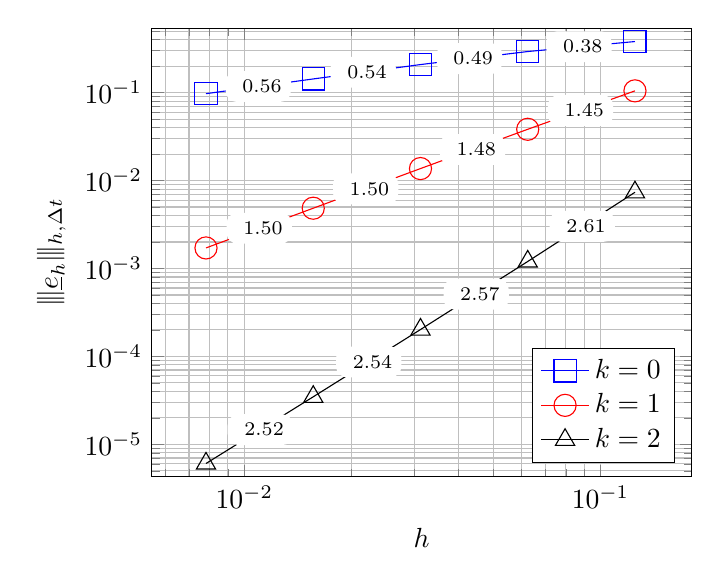
\begin{tikzpicture}
\begin{axis}[xmin=   5.5E-03, xmax=   1.8E-01, xmode=log, log basis x=10, xlabel=$h$,
             ymin=   4.3E-06, ymax=   5.4E-01, ymode=log, log basis y=10, ylabel=$\tnorm{h,\Delta t}{\underline{e}_h}$,
             axis background/.style={fill=gray!0},
             legend pos=south east,
             grid=both]
% Plot k = 0
\addplot[color=blue, mark=square, mark options={scale=2}] coordinates {
(     1.25000E-01 ,     3.81054E-01 )
(     6.25000E-02 ,     2.93360E-01 )
(     3.12500E-02 ,     2.08490E-01 )
(     1.56250E-02 ,     1.43095E-01 )
(     7.81250E-03 ,     9.72830E-02 ) }
node[pos= 0.125, fill=white, text=black, rounded corners] {\contour{white}{\scriptsize{  0.38}}}
node[pos= 0.375, fill=white, text=black, rounded corners] {\contour{white}{\scriptsize{  0.49}}}
node[pos= 0.625, fill=white, text=black, rounded corners] {\contour{white}{\scriptsize{  0.54}}}
node[pos= 0.875, fill=white, text=black, rounded corners] {\contour{white}{\scriptsize{  0.56}}};

% Plot k = 1
\addplot[color=red, mark=o, mark options={scale=2}] coordinates {
(     1.25000E-01 ,     1.04741E-01 )
(     6.25000E-02 ,     3.82962E-02 )
(     3.12500E-02 ,     1.36859E-02 )
(     1.56250E-02 ,     4.84648E-03 )
(     7.81250E-03 ,     1.71241E-03 ) }
node[pos= 0.125, fill=white, text=black, rounded corners] {\contour{white}{\scriptsize{  1.45}}}
node[pos= 0.375, fill=white, text=black, rounded corners] {\contour{white}{\scriptsize{  1.48}}}
node[pos= 0.625, fill=white, text=black, rounded corners] {\contour{white}{\scriptsize{  1.50}}}
node[pos= 0.875, fill=white, text=black, rounded corners] {\contour{white}{\scriptsize{  1.50}}};

% Plot k = 2
\addplot[color=black, mark=triangle, mark options={scale=2}] coordinates {
(     1.25000E-01 ,     7.35406E-03 )
(     6.25000E-02 ,     1.20104E-03 )
(     3.12500E-02 ,     2.02092E-04 )
(     1.56250E-02 ,     3.47347E-05 )
(     7.81250E-03 ,     6.05252E-06 ) }
node[pos= 0.125, fill=white, text=black, rounded corners] {\contour{white}{\scriptsize{  2.61}}}
node[pos= 0.375, fill=white, text=black, rounded corners] {\contour{white}{\scriptsize{  2.57}}}
node[pos= 0.625, fill=white, text=black, rounded corners] {\contour{white}{\scriptsize{  2.54}}}
node[pos= 0.875, fill=white, text=black, rounded corners] {\contour{white}{\scriptsize{  2.52}}};

% Legend
\legend{
{$k= 0$},
{$k= 1$},
{$k= 2$}
};
\end{axis}
\end{tikzpicture}
}
\caption{$\nu=10^{-6}$}
\end{subfigure}

	~
	\begin{subfigure}[b]{0.45\textwidth}
\centering
\resizebox{\textwidth}{!}{
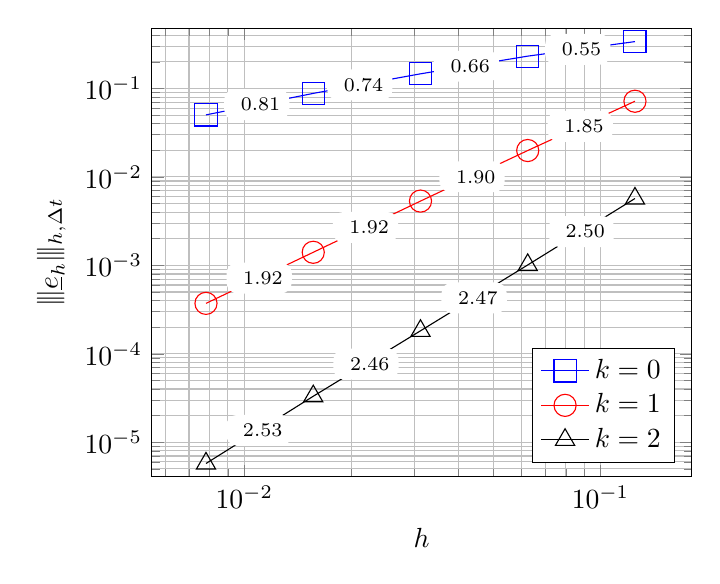
\begin{tikzpicture}
\begin{axis}[xmin=   5.5E-03, xmax=   1.8E-01, xmode=log, log basis x=10, xlabel=$h$,
             ymin=   4.1E-06, ymax=   4.8E-01, ymode=log, log basis y=10, ylabel=$\tnorm{h,\Delta t}{\underline{e}_h}$,
             axis background/.style={fill=gray!0},
             legend pos=south east,
             grid=both]
% Plot k = 0
\addplot[color=blue, mark=square, mark options={scale=2}] coordinates {
(     1.25000E-01 ,     3.38889E-01 )
(     6.25000E-02 ,     2.32091E-01 )
(     3.12500E-02 ,     1.46516E-01 )
(     1.56250E-02 ,     8.80178E-02 )
(     7.81250E-03 ,     5.03008E-02 ) }
node[pos= 0.125, fill=white, text=black, rounded corners] {\contour{white}{\scriptsize{  0.55}}}
node[pos= 0.375, fill=white, text=black, rounded corners] {\contour{white}{\scriptsize{  0.66}}}
node[pos= 0.625, fill=white, text=black, rounded corners] {\contour{white}{\scriptsize{  0.74}}}
node[pos= 0.875, fill=white, text=black, rounded corners] {\contour{white}{\scriptsize{  0.81}}};

% Plot k = 1
\addplot[color=red, mark=o, mark options={scale=2}] coordinates {
(     1.25000E-01 ,     7.17646E-02 )
(     6.25000E-02 ,     1.98930E-02 )
(     3.12500E-02 ,     5.33458E-03 )
(     1.56250E-02 ,     1.40692E-03 )
(     7.81250E-03 ,     3.72283E-04 ) }
node[pos= 0.125, fill=white, text=black, rounded corners] {\contour{white}{\scriptsize{  1.85}}}
node[pos= 0.375, fill=white, text=black, rounded corners] {\contour{white}{\scriptsize{  1.90}}}
node[pos= 0.625, fill=white, text=black, rounded corners] {\contour{white}{\scriptsize{  1.92}}}
node[pos= 0.875, fill=white, text=black, rounded corners] {\contour{white}{\scriptsize{  1.92}}};

% Plot k = 2
\addplot[color=black, mark=triangle, mark options={scale=2}] coordinates {
(     1.25000E-01 ,     5.70534E-03 )
(     6.25000E-02 ,     1.01148E-03 )
(     3.12500E-02 ,     1.82183E-04 )
(     1.56250E-02 ,     3.31678E-05 )
(     7.81250E-03 ,     5.76220E-06 ) }
node[pos= 0.125, fill=white, text=black, rounded corners] {\contour{white}{\scriptsize{  2.50}}}
node[pos= 0.375, fill=white, text=black, rounded corners] {\contour{white}{\scriptsize{  2.47}}}
node[pos= 0.625, fill=white, text=black, rounded corners] {\contour{white}{\scriptsize{  2.46}}}
node[pos= 0.875, fill=white, text=black, rounded corners] {\contour{white}{\scriptsize{  2.53}}};

% Legend
\legend{
{$k= 0$},
{$k= 1$},
{$k= 2$}
};
\end{axis}
\end{tikzpicture}
}
\caption{$\nu=10^{-2}$}
\end{subfigure}

	\
	\begin{subfigure}[b]{0.45\textwidth}
\centering
\resizebox{\textwidth}{!}{
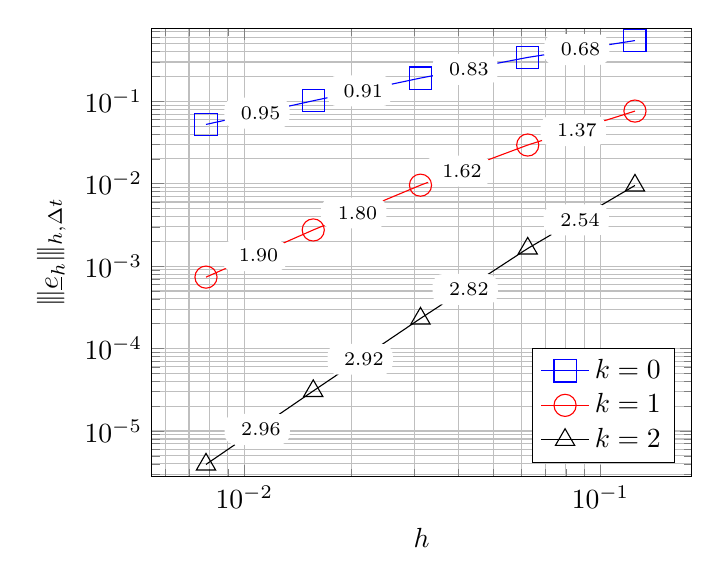
\begin{tikzpicture}
\begin{axis}[xmin=   5.5E-03, xmax=   1.8E-01, xmode=log, log basis x=10, xlabel=$h$,
             ymin=   2.8E-06, ymax=   7.7E-01, ymode=log, log basis y=10, ylabel=$\tnorm{h,\Delta t}{\underline{e}_h}$,
             axis background/.style={fill=gray!0},
             legend pos=south east,
             grid=both]
% Plot k = 0
\addplot[color=blue, mark=square, mark options={scale=2}] coordinates {
(     1.25000E-01 ,     5.45283E-01 )
(     6.25000E-02 ,     3.40638E-01 )
(     3.12500E-02 ,     1.91337E-01 )
(     1.56250E-02 ,     1.01479E-01 )
(     7.81250E-03 ,     5.23723E-02 ) }
node[pos= 0.125, fill=white, text=black, rounded corners] {\contour{white}{\scriptsize{  0.68}}}
node[pos= 0.375, fill=white, text=black, rounded corners] {\contour{white}{\scriptsize{  0.83}}}
node[pos= 0.625, fill=white, text=black, rounded corners] {\contour{white}{\scriptsize{  0.91}}}
node[pos= 0.875, fill=white, text=black, rounded corners] {\contour{white}{\scriptsize{  0.95}}};

% Plot k = 1
\addplot[color=red, mark=o, mark options={scale=2}] coordinates {
(     1.25000E-01 ,     7.60798E-02 )
(     6.25000E-02 ,     2.94772E-02 )
(     3.12500E-02 ,     9.59876E-03 )
(     1.56250E-02 ,     2.74824E-03 )
(     7.81250E-03 ,     7.35890E-04 ) }
node[pos= 0.125, fill=white, text=black, rounded corners] {\contour{white}{\scriptsize{  1.37}}}
node[pos= 0.375, fill=white, text=black, rounded corners] {\contour{white}{\scriptsize{  1.62}}}
node[pos= 0.625, fill=white, text=black, rounded corners] {\contour{white}{\scriptsize{  1.80}}}
node[pos= 0.875, fill=white, text=black, rounded corners] {\contour{white}{\scriptsize{  1.90}}};

% Plot k = 2
\addplot[color=black, mark=triangle, mark options={scale=2}] coordinates {
(     1.25000E-01 ,     9.52371E-03 )
(     6.25000E-02 ,     1.63804E-03 )
(     3.12500E-02 ,     2.31856E-04 )
(     1.56250E-02 ,     3.06028E-05 )
(     7.81250E-03 ,     3.92850E-06 ) }
node[pos= 0.125, fill=white, text=black, rounded corners] {\contour{white}{\scriptsize{  2.54}}}
node[pos= 0.375, fill=white, text=black, rounded corners] {\contour{white}{\scriptsize{  2.82}}}
node[pos= 0.625, fill=white, text=black, rounded corners] {\contour{white}{\scriptsize{  2.92}}}
node[pos= 0.875, fill=white, text=black, rounded corners] {\contour{white}{\scriptsize{  2.96}}};

% Legend
\legend{
{$k= 0$},
{$k= 1$},
{$k= 2$}
};
\end{axis}
\end{tikzpicture}
}
\caption{$\nu=10^{-1}$}
\end{subfigure}

	~
	\begin{subfigure}[b]{0.45\textwidth}
\centering
\resizebox{\textwidth}{!}{
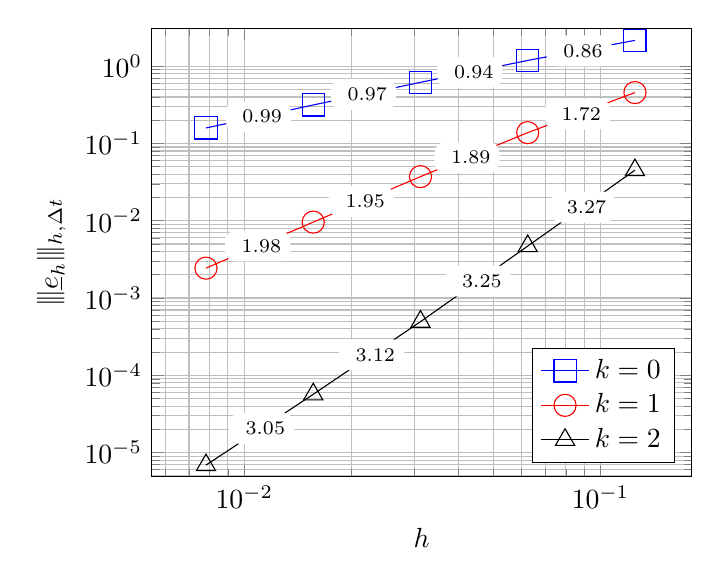
\begin{tikzpicture}
\begin{axis}[xmin=   5.5E-03, xmax=   1.8E-01, xmode=log, log basis x=10, xlabel=$h$,
             ymin=   4.9E-06, ymax=   3.1E+00, ymode=log, log basis y=10, ylabel=$\tnorm{h,\Delta t}{\underline{e}_h}$,
             axis background/.style={fill=gray!0},
             legend pos=south east,
             grid=both]
% Plot k = 0
\addplot[color=blue, mark=square, mark options={scale=2}] coordinates {
(     1.25000E-01 ,     2.15984E+00 )
(     6.25000E-02 ,     1.18719E+00 )
(     3.12500E-02 ,     6.18504E-01 )
(     1.56250E-02 ,     3.14932E-01 )
(     7.81250E-03 ,     1.58786E-01 ) }
node[pos= 0.125, fill=white, text=black, rounded corners] {\contour{white}{\scriptsize{  0.86}}}
node[pos= 0.375, fill=white, text=black, rounded corners] {\contour{white}{\scriptsize{  0.94}}}
node[pos= 0.625, fill=white, text=black, rounded corners] {\contour{white}{\scriptsize{  0.97}}}
node[pos= 0.875, fill=white, text=black, rounded corners] {\contour{white}{\scriptsize{  0.99}}};

% Plot k = 1
\addplot[color=red, mark=o, mark options={scale=2}] coordinates {
(     1.25000E-01 ,     4.55963E-01 )
(     6.25000E-02 ,     1.38136E-01 )
(     3.12500E-02 ,     3.72359E-02 )
(     1.56250E-02 ,     9.60828E-03 )
(     7.81250E-03 ,     2.43670E-03 ) }
node[pos= 0.125, fill=white, text=black, rounded corners] {\contour{white}{\scriptsize{  1.72}}}
node[pos= 0.375, fill=white, text=black, rounded corners] {\contour{white}{\scriptsize{  1.89}}}
node[pos= 0.625, fill=white, text=black, rounded corners] {\contour{white}{\scriptsize{  1.95}}}
node[pos= 0.875, fill=white, text=black, rounded corners] {\contour{white}{\scriptsize{  1.98}}};

% Plot k = 2
\addplot[color=black, mark=triangle, mark options={scale=2}] coordinates {
(     1.25000E-01 ,     4.52028E-02 )
(     6.25000E-02 ,     4.69922E-03 )
(     3.12500E-02 ,     4.94384E-04 )
(     1.56250E-02 ,     5.68190E-05 )
(     7.81250E-03 ,     6.88133E-06 ) }
node[pos= 0.125, fill=white, text=black, rounded corners] {\contour{white}{\scriptsize{  3.27}}}
node[pos= 0.375, fill=white, text=black, rounded corners] {\contour{white}{\scriptsize{  3.25}}}
node[pos= 0.625, fill=white, text=black, rounded corners] {\contour{white}{\scriptsize{  3.12}}}
node[pos= 0.875, fill=white, text=black, rounded corners] {\contour{white}{\scriptsize{  3.05}}};

% Legend
\legend{
{$k= 0$},
{$k= 1$},
{$k= 2$}
};
\end{axis}
\end{tikzpicture}
}
\caption{$\nu=10^{0}$}
\end{subfigure}

	\caption{Convergence rates for the numerical tests of Section \ref{sec:num} with $\nu\in\{10^{-6},10^{-2},10^{-1},1\}$ and $k\in\{0,1,2\}$. Estimated orders of convergence between successive spatial $h$-refinements are also given.}
	\label{fig:convergence:tnorm}
\end{figure}

%% Please add the following required packages to your document preamble:
% \usepackage[table,xcdraw]{xcolor}
% If you use beamer only pass "xcolor=table" option, i.e. \documentclass[xcolor=table]{beamer}
\begin{table}[]
\begin{tabular}{lllllll}
                                                                                                                     & Storyline Development Stage &                       & Character Design Stage &                        & Character Drawing Stage &                       \\
\multicolumn{7}{c}{\cellcolor[HTML]{D9D9D9}Needs \& Challenges}                                                                                                                                                                                                                \\
                                                                                                                     & Needs                       & Challenges            & Needs                  & Challenges             & Needs                   & Challenges            \\
gauge reader reactions                                                                                               & \multicolumn{1}{r}{3}       &                       &                        & \multicolumn{1}{r}{3}  &                         &                       \\
organize the story flow                                                                                              & \multicolumn{1}{r}{3}       & \multicolumn{1}{r}{4} &                        &                        &                         &                       \\
find interesting story sources that could captivate readers’ interest                                                & \multicolumn{1}{r}{2}       & \multicolumn{1}{r}{4} &                        &                        &                         &                       \\
struggled with creating a story                                                                                      &                             & \multicolumn{1}{r}{8} &                        &                        &                         &                       \\
maintaining a consistent storyline regardless of their condition                                                     &                             & \multicolumn{1}{r}{1} &                        &                        &                         &                       \\
get feedback from readers                                                                                            &                             &                       & \multicolumn{1}{r}{2}  &                        &                         &                       \\
get specific design ideas                                                                                            &                             &                       & \multicolumn{1}{r}{1}  &                        &                         &                       \\
uniqueness of their characters                                                                                       &                             &                       & \multicolumn{1}{r}{4}  & \multicolumn{1}{r}{10} &                         &                       \\
\begin{tabular}[c]{@{}l@{}}enhance the efficiency in their\\ work process by improving repetitive tasks\end{tabular} &                             &                       &                        &                        & \multicolumn{1}{r}{7}   &                       \\
receive materials related to composition                                                                             &                             &                       &                        &                        & \multicolumn{1}{r}{4}   &                       \\
provided to research reference materials                                                                             &                             &                       &                        &                        & \multicolumn{1}{r}{1}   &                       \\
struggled with drawing characters in a variety of compositions                                                       &                             &                       &                        &                        &                         & \multicolumn{1}{r}{6} \\
limited drawinig skills                                                                                              &                             &                       &                        &                        &                         & \multicolumn{1}{r}{6} \\
get information that could be used as reference material                                                             & \multicolumn{1}{r}{2}       &                       & \multicolumn{1}{r}{6}  & \multicolumn{1}{r}{2}  & \multicolumn{1}{r}{1}   &                       \\
\multicolumn{7}{c}{\cellcolor[HTML]{D9D9D9}Expectations}                                                                                                                                                                                                                       \\
Expectations for Generating Ideas                                                                                    & \multicolumn{1}{r}{9}       &                       & \multicolumn{1}{r}{11} &                        & \multicolumn{1}{r}{1}   &                       \\
Expectations for Receiving References from AI                                                                        & \multicolumn{1}{r}{4}       &                       & \multicolumn{1}{r}{0}  &                        & \multicolumn{1}{r}{5}   &                       \\
Expectations of rapid visualization using AI                                                                         & \multicolumn{1}{r}{0}       &                       & \multicolumn{1}{r}{2}  &                        & \multicolumn{1}{r}{2}   &                       \\
\multicolumn{7}{c}{\cellcolor[HTML]{D9D9D9}Considerations}                                                                                                                                                                                                                     \\
Skepticism Regarding AI Capabilities                                                                                 & \multicolumn{1}{r}{2}       &                       & \multicolumn{1}{r}{3}  &                        & \multicolumn{1}{r}{0}   &                       \\
Refusal to Use AI Due to Copyright Infringement and Concerns About the Author's Identity                             & \multicolumn{1}{r}{3}       &                       & \multicolumn{1}{r}{1}  &                        & \multicolumn{1}{r}{2}   &                       \\
Low Utility of AI Outputs                                                                                            & \multicolumn{1}{r}{3}       &                       & \multicolumn{1}{r}{1}  &                        & \multicolumn{1}{r}{1}   &                      
\end{tabular}
\end{table}

%Table \ref{tab:convergence:components} shows how the error $\tnorm{h,\Delta_t}{\underline{e}_h}$ breaks down into its discrete-$L^\infty(L^2)$, viscous and jump components. In the convection-dominated case, the jump seminorm $\seminorm{\beta,h,\Delta t}{\underline{e}_h}$ provides the dominant contribution to $\tnorm{h,\Delta t}{\underline{e}_h}$ and converges with rate $k+\frac12$, whereas the viscous norm $\norm{\nu,h,\Delta t}{\underline{e}_h}$ provides the dominant contribution to $\tnorm{h,\Delta t}{\underline{e}_h}$ and converges with rate $k+1$ in the diffusion-dominated case. Interestingly, the jump seminorm appears to superconverge in the diffusion-dominated case with convergence rate $k+\frac32$.

%------------------------------------------------------------------------------%

\section*{Acknowledgements}

Funded by the European Union (ERC Synergy, NEMESIS, project number 101115663).
Views and opinions expressed are however those of the authors only and do not necessarily reflect those of the European Union or the European Research Council Executive Agency. Neither the European Union nor the granting authority can be held responsible for them.

%------------------------------------------------------------------------------%

\printbibliography

\end{document}

%%%%%%%%%%%%%%%%%%%%%%%%%%%%%%%%%%%%%%%%
     ERASED TABLE (remark on variants)
%%%%%%%%%%%%%%%%%%%%%%%%%%%%%%%%%%%%%%%%

\begin{table}[h]
    \centering
    \begin{tabular}{lccc}
        \toprule
        Method & Diffusion-dominated & Advection-dominated & Notes \\  
        \midrule 
        Choice 1  & $h^{k+1}$ & $h^{k+ \frac12}$ & Modify \eqref{eq:tT} and $j_{\beta,h}$ \\
        Choice 2  & $h^{k+1}$ & $h^{k+ \frac12}$ & - \\
        \bottomrule
    \end{tabular}
    \caption{Summary of the convergence rates for each scenario, in both the diffusion- and advection-dominated regimes (cf. Lemma \ref{cor:convergence.rate}).}
    \label{tab:bmd_scenarios_resume}
\end{table}
